\documentclass[../notes.tex]{subfiles}

\pagestyle{main}
\renewcommand{\chaptermark}[1]{\markboth{\chaptername\ \thechapter\ (#1)}{}}
\setcounter{chapter}{6}

\begin{document}




\chapter{Gas-Phase Product Molecule Analysis and Intro to Lattices}
\section{Directional Scattering of the Product Molecule}
\begin{itemize}
    \item \marginnote{5/9:}The velocity and angular distribution of the products of a reactive collision.
    \begin{itemize}
        \item We have that
        \begin{align*}
            E_\text{trans}'+E_\text{vib}' &= E_\text{trans}+E_\text{vib}-[D_e(\ce{D2})-D_e(\ce{DF})]\\
            &= \SI{7.62}{\kilo\joule\per\mole}+\SI{17.9}{\kilo\joule\per\mole}+\SI{140}{\kilo\joule\per\mole}\\
            &= \SI{166}{\kilo\joule\per\mole}
        \end{align*}
        \item Additionally, we know that
        \begin{equation*}
            E_\text{trans}'+E_\text{vib}' = \frac{1}{2}\mu'u_r'^2+(\SI{34.8}{\kilo\joule\per\mole})\left( v+\frac{1}{2} \right)
            = \SI{166}{\kilo\joule\per\mole}
        \end{equation*}
        \item The relationship between the vibrational quantum number, the relative speed of the products, and the speed of \ce{DF} relative to the center of mass has been tabulated.
    \end{itemize}
    \item A contour map of the angular and speed distributions for the product molecule.
    \begin{itemize}
        \item The contour plot.
        \begin{itemize}
            \item The center of mass is fixed at the origin.
            \item The dashed circles correspond to the maximum relative speeds a \ce{DF} molecule can have for the indicated vibrational state.
            \item The product molecules preferentially scatter back in the direction of the incident fluorine atom, a scattering angle of $\theta=\ang{180}$.
            \item The arrows at the bottom of the figure show the direction with which each reactant molecule approaches the other.
        \end{itemize}
        \item Another picture is provided, illustrating the atom-molecule reaction \ce{F + D2} in which $\theta=\ang{0}$ and $\theta=\ang{180}$.
        \item The influence of rotation.
        \begin{itemize}
            \item Large numbers of product molecules have speeds between the dashed circles.
            \item The dash circles correspond to the case where there is internal energy only in the vibrational states of the molecule, in which case the rotational energy corresponding to these circles is $E_\text{rot}=0$ with $J=0$.
            \item If \ce{DF} is produced in an excited rotational state, we would expect to observe a speed that has a value intermediate between two fo the dashed circles.
        \end{itemize}
    \end{itemize}
    \item Not all gas-phase chemical reactions are rebound reactions.
    \begin{itemize}
        \item Consider the reaction
        \begin{equation*}
            \ce{K(g) + I2(g) -> KI(g) + I(g)}
        \end{equation*}
        \begin{itemize}
            \item The product diatomic molecule in this case (\ce{KI}) is preferentially scattered in the forward direction along the direction of the incident \ce{K} atom.
        \end{itemize}
        \item Consider the reaction
        \begin{equation*}
            \ce{O(g) + Br2(g)} \Longrightarrow \ce{BrO(g) + Br(g)}
        \end{equation*}
        \begin{itemize}
            \item The product molecule \ce{BrO} is forward and back scattered with equal intensity.
        \end{itemize}
        \item Both of these observations can be read off of the contour maps of the two reactions.
    \end{itemize}
\end{itemize}



\section{Potential Energy Surfaces}
\begin{itemize}
    \item \marginnote{5/11:}The velocity and angular distribution of the products of a reactive collision.
    \begin{figure}[h!]
        \centering
        \begin{tikzpicture}
            \footnotesize
            \draw [dashed] (-5.5,0) -- (-0.18,0) (5.5,0) -- (0.18,0);
    
            \draw
                (-4,0) ellipse (7mm and 1.5cm) node[above=2cm,align=center]{Approaching\\reactant}
                (4,0) ellipse (1.05cm and 2.25cm) node[above=2.75cm,align=center]{Leaving\\product}
            ;
            \draw
                (-4,0) ++(145:1.5) ++(0.65,0) coordinate(A) -- (-4,0)
                (-4,0) ++(20:1.5) ++(-0.75,0) coordinate (A') -- (-4,0)
                ($(-4,0)!0.3!(A)$) arc[start angle=150,end angle=18,x radius=2.1mm,y radius=4.5mm]
                ($(-4,0)!0.25!(A')$) -- ++(0.25,0) -- (-3.75,0)
            ;
            \node at (-4,0.65) {$\phi$};
            \draw
                (4,0) ++(145:2.25) ++(0.98,0) coordinate(C) -- (4,0)
                (4,0) ++(20:2.25) ++(-1.13,0) coordinate (C') -- (4,0)
                ($(4,0)!0.2!(C)$) arc[start angle=150,end angle=18,x radius=2.1mm,y radius=4.5mm]
                ($(4,0)!0.17!(C')$) -- ++(0.25,0) -- (4.25,0)
            ;
            \node at (4,0.65) {$\phi$};
    
            \draw [semithick,-latex] (A) -- node[above]{$\mathbf{u}_r$} (A -| 0,0) -- node[above]{$\mathbf{u}_r'$} ($(A -| 0,0)!0.84!(C)$);
            \draw (A -| -0.45,0) arc[start angle=180,end angle=8,radius=4.5mm];
            \node [fill=white,inner sep=1.5pt] at ([yshift=4.5mm]A -| 0,0) {$\theta$};
    
            \draw [<->,shorten <=1pt,shorten >=1pt] (-2,0 |- A) -- node[right]{$b$} (-2,0);
    
            \begin{scope}[on background layer]
                \fill [ball color=rex] (0,0) circle (1cm) node{\ce{B}};
                \fill [ball color=blx] (A) circle (5mm) node[left]{\ce{A}};
                \fill [ball color=blx] (C) circle (5mm);
            \end{scope}
        \end{tikzpicture}
        \caption{Velocity and angular distributions of the products.}
        \label{fig:velocityAngleDist}
    \end{figure}
    \begin{itemize}
        \item For a fixed value of the impact parameter $b$, the reactants and products take on all possible angles $\phi$ with equal probability, thereby forming a cone around the relative velocity vector $\mathbf{u}_r$.
        \item The angle $\theta$, however, depends on the dynamics of the reaction and must be determined experimentally.
    \end{itemize}
    \item The potential energy of a polyatomic molecule depends on more than one variable.
    \begin{itemize}
        \item \ce{D2}.
        \begin{itemize}
            \item Consider the potential energy curve of \ce{D2}. The zero of energy is defined to be that of the two separated atoms. The minimum of the potential energy curve corresponds to the equilibrium bond length of the \ce{D2} molecule.
        \end{itemize}
        \item \ce{H2O}.
        \begin{itemize}
            \item The potential energy of a water molecule is a function of the three parameters $r_{\ce{O-H_A}}$, $r_{\ce{O-H_B}}$, and $\alpha$ (two bond lengths and the interbond angle). In an equation,
            \begin{equation*}
                V = V(r_{\ce{O-H_A}},r_{\ce{O-H_B}},\alpha)
            \end{equation*}
            \item A plot of the complete potential energy surface of a water molecule therefore requires four axes.
        \end{itemize}
    \end{itemize}
    \item The potential energy of a chemical reaction depends on more than one variable.
    \begin{figure}[H]
        \centering
        \footnotesize
        \begin{subfigure}[b]{0.3\linewidth}
            \centering
            \begin{tikzpicture}
                \node (DA) at (0,0)   {\ce{D_A}};
                \node (DB) at (1.3,0) {\ce{D_B}};
                \node (F)  at (180:2) {\ce{F}};
    
                \draw [semithick,dashed] (F)  -- node[above]{$\beta=\ang{180}$} (DA);
                \draw [semithick] (DA) -- (DB);
            \end{tikzpicture}
            \caption{Linear.}
            \label{fig:FD2attackAnglea}
        \end{subfigure}
        \begin{subfigure}[b]{0.3\linewidth}
            \centering
            \begin{tikzpicture}
                \node (DA) at (0,0)   {\ce{D_A}};
                \node (DB) at (1.3,0) {\ce{D_B}};
                \node (F)  at (135:2) {\ce{F}};
    
                \draw [semithick,dashed] (F)  -- node[above right]{$\beta=\ang{180}$} (DA);
                \draw [semithick] (DA) -- (DB);
            \end{tikzpicture}
            \caption{Bent.}
            \label{fig:FD2attackAngleb}
        \end{subfigure}
        \begin{subfigure}[b]{0.3\linewidth}
            \centering
            \begin{tikzpicture}
                \node (DA) at (0,0)   {\ce{D_A}};
                \node (DB) at (1.3,0) {\ce{D_B}};
                \node (F)  at (90:2) {\ce{F}};
    
                \draw [semithick,dashed] (F)  -- node[right]{$\beta=\ang{180}$} (DA);
                \draw [semithick] (DA) -- (DB);
            \end{tikzpicture}
            \caption{Perpendicular.}
            \label{fig:FD2attackAnglec}
        \end{subfigure}
        \caption{Angle of attack in \ce{F + D2}.}
        \label{fig:FD2attackAngle}
    \end{figure}
    \begin{itemize}
        \item Consider, once again, the reaction
        \begin{equation*}
            \ce{F(g) + D_AD_B(g)} \Longrightarrow \ce{D_AF(g) + D_B(g)}
        \end{equation*}
        \item When the reactants are at infinite separation, there are no attractive or repulsive forces between the fluorine atom and the \ce{D2} molecule, so the potential energy surface for the reaction is the same as that for an isolated \ce{D2} molecule.
        \item Likewise, when the products are at infinite separation, the potential-energy surface for the reaction is the same as the for the isolated \ce{DF} molecule.
        \item As the reaction occurs, however, the distance between the fluroine atom and \ce{D_A} decreases and the distance between \ce{D_A} and \ce{D_B} increases, and the potential energy depends on both distances.
        \item The potential energy also depends on the angle at which the \ce{F} atom approaches the \ce{D2} molecule.
    \end{itemize}
    \item As with the angular and speed distributions, we can draw an energy contour map for the reaction.
    \begin{itemize}
        \item The zero of energy is defined as the infinitely separated reactants. Point B is the location of the transition state of the reaction.
    \end{itemize}
    \item Tian does a brief summary of Chapter 30.
\end{itemize}



\section{Lattice Structure}
\begin{itemize}
    \item \marginnote{5/13:}The unit cell is the fundamental building block of a crystal.
    \begin{itemize}
        \item We can think of a crystal as a two- or three-dimensional lattice.
        \item Either way, we can identify blocks in the lattice that form a regularly repeating structure.
    \end{itemize}
    \item \textbf{Face-centered cubic} (unit cell): The following unit cell. \emph{Also known as} \textbf{FCC}, \textbf{cubic close-packing}. \emph{Structure}
    \begin{figure}[H]
        \centering
        \begin{subfigure}[b]{0.2\linewidth}
            \centering
            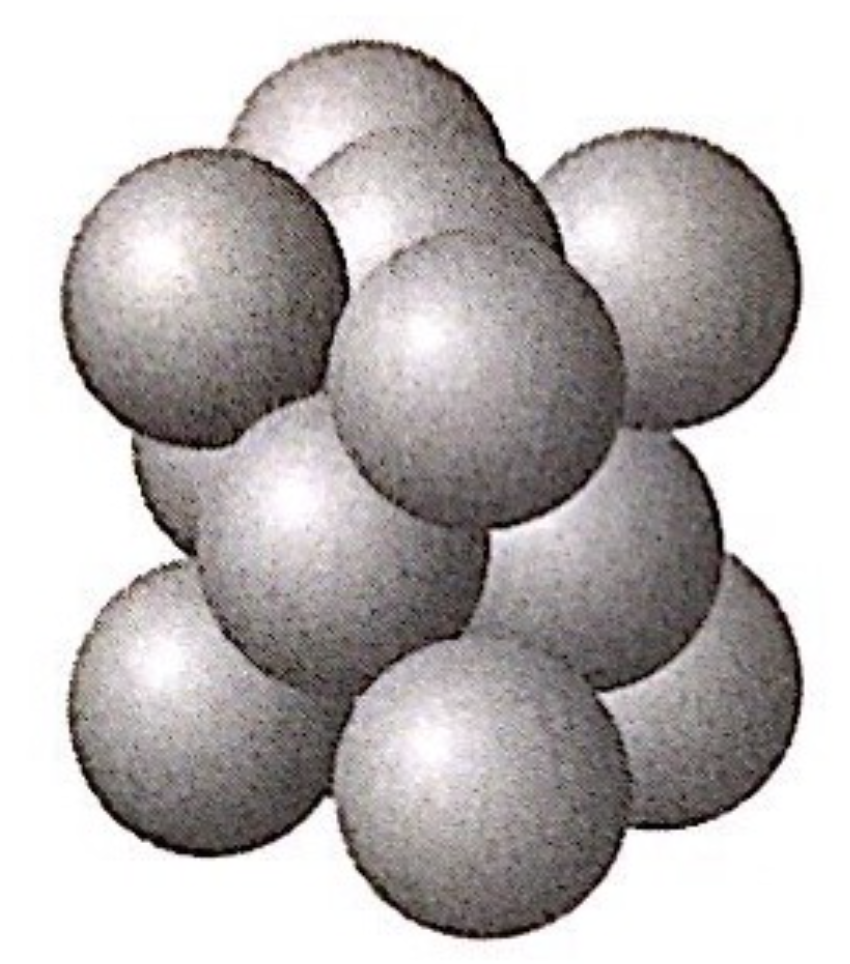
\includegraphics[width=0.6\linewidth]{../ExtFiles/FCCunitCella.png}
            \caption{Atomic picture.}
            \label{fig:FCCunitCella}
        \end{subfigure}
        \begin{subfigure}[b]{0.2\linewidth}
            \centering
            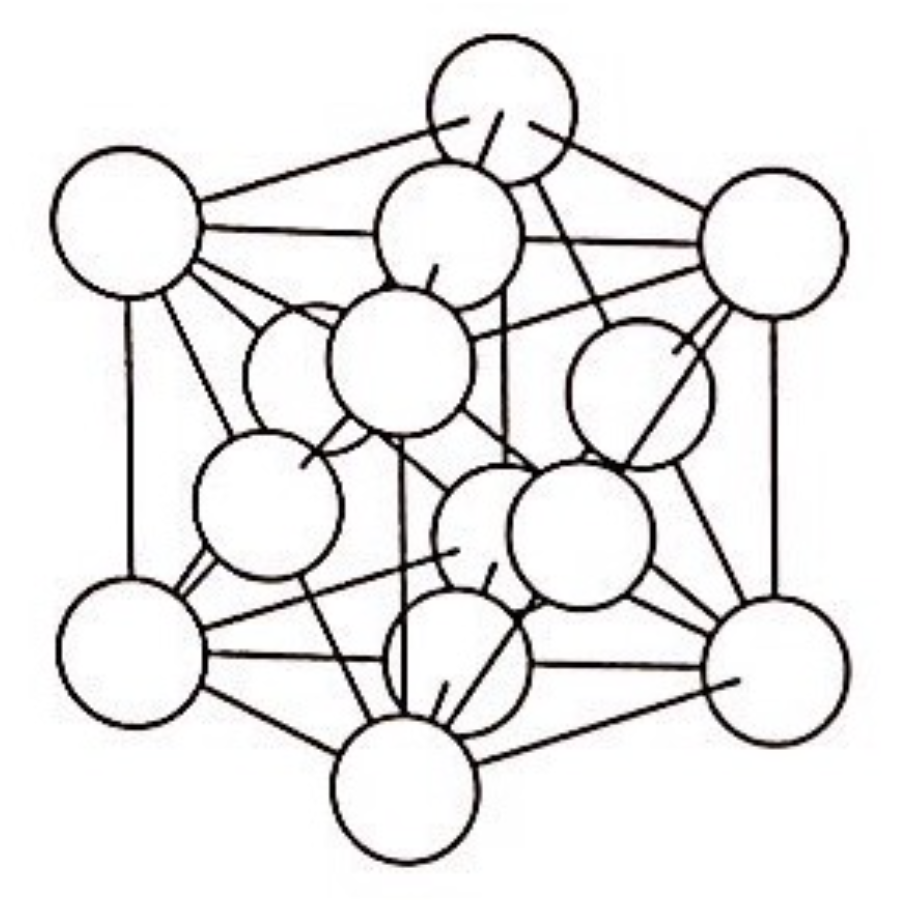
\includegraphics[width=0.7\linewidth]{../ExtFiles/FCCunitCellb.png}
            \caption{Lattice picture.}
            \label{fig:FCCunitCellb}
        \end{subfigure}
        \begin{subfigure}[b]{0.2\linewidth}
            \centering
            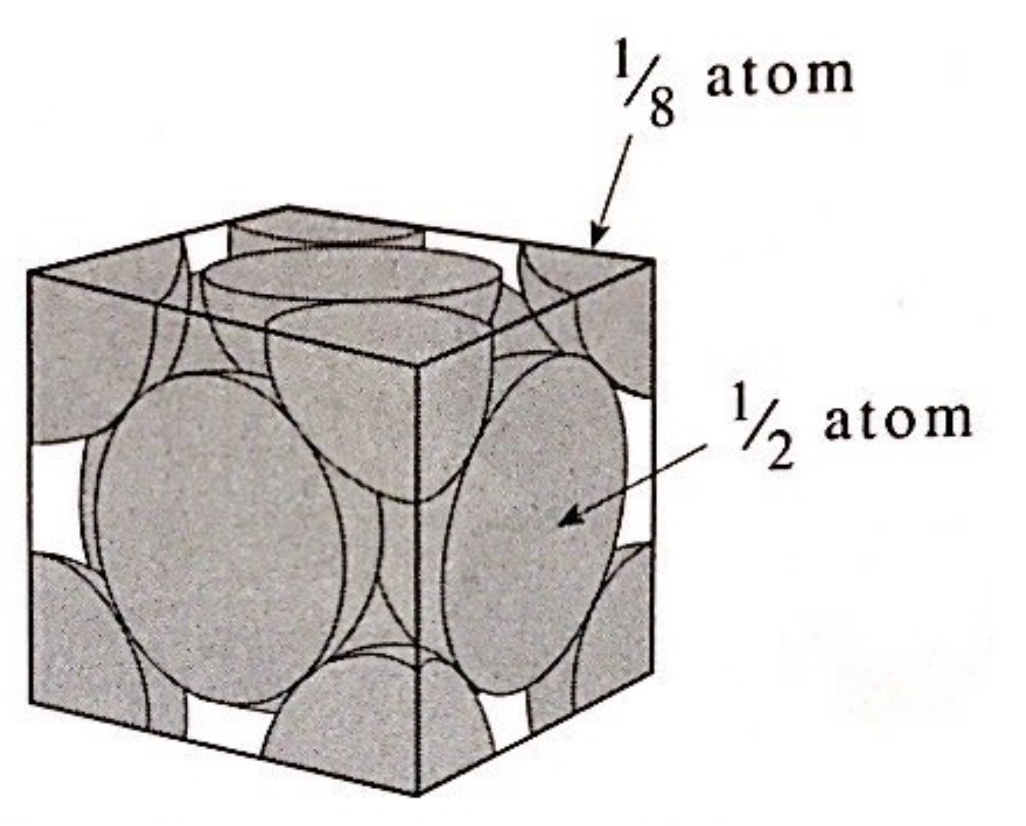
\includegraphics[width=1.0\linewidth]{../ExtFiles/FCCunitCellc.png}
            \caption{Unit cell.}
            \label{fig:FCCunitCellc}
        \end{subfigure}
        \caption{Face-centered cubic unit cell.}
        \label{fig:FCCunitCell}
    \end{figure}
    \begin{itemize}
        \item Figure \ref{fig:FCCunitCella} shows the set of atoms that contribute to a unit cell of the crystal. The unit cell, itself, is a cube however (see Figure \ref{fig:FCCunitCellc}).
        \item Figure \ref{fig:FCCunitCellb} shows the unit cell for a three-dimensional lattice model of copper, where each point of the crystal is associated with a lattice point.
        \item Figure \ref{fig:FCCunitCellc} shows the fractions of each copper atom shown in Figure \ref{fig:FCCunitCella} that contribute to the unit cell of the crystal.
        \item There are four atoms per unit cell (six half-atoms and eight eighth-atoms).
        \item Example: The packing of copper atoms in a copper crystal gives a face-centered cubic unit cell.
    \end{itemize}
    \item \textbf{Body-centered cubic} (unit cell): The following unit cell. \emph{Also known as} \textbf{BCC}. \emph{Structure}
    \begin{figure}[h!]
        \centering
        \begin{subfigure}[b]{0.2\linewidth}
            \centering
            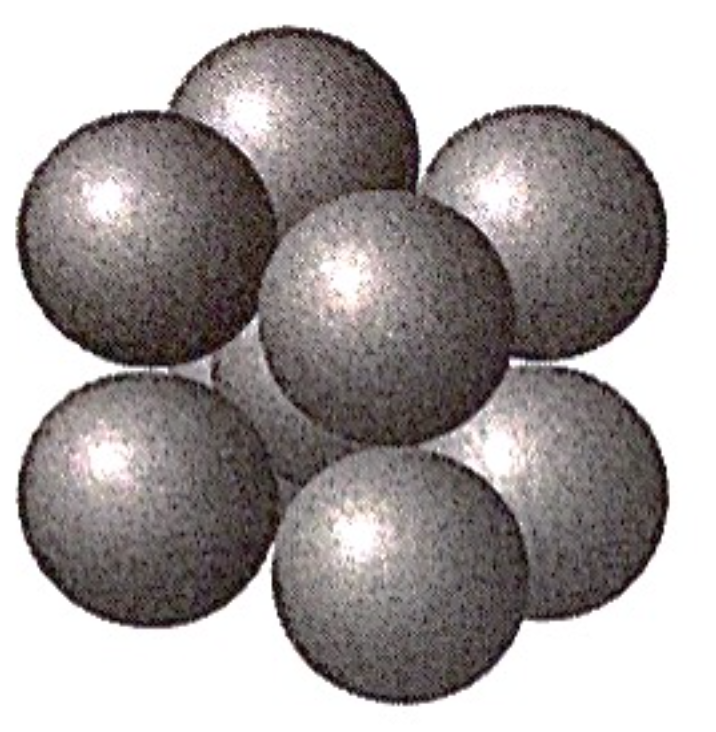
\includegraphics[width=0.6\linewidth]{../ExtFiles/BCCunitCella.png}
            \caption{Atomic picture.}
            \label{fig:BCCunitCella}
        \end{subfigure}
        \begin{subfigure}[b]{0.2\linewidth}
            \centering
            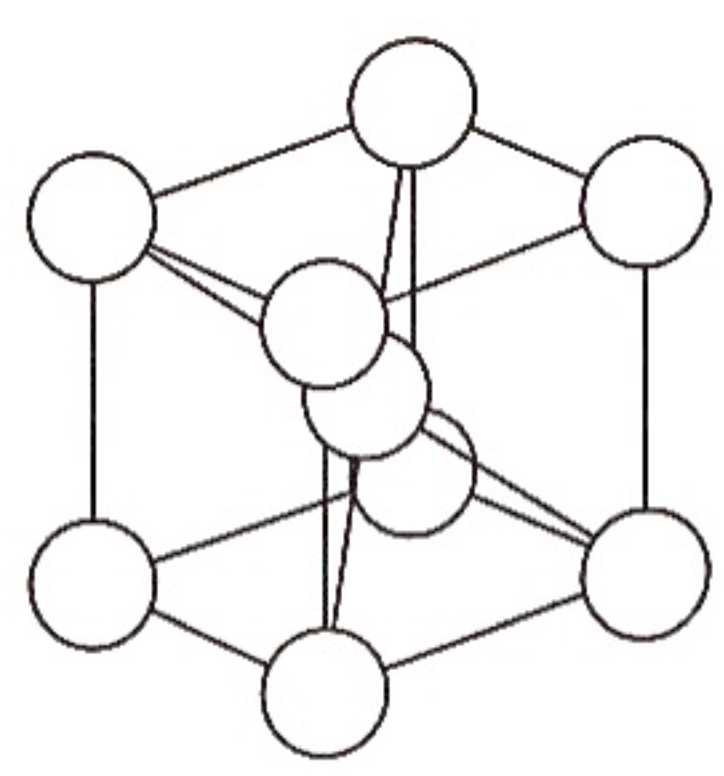
\includegraphics[width=0.65\linewidth]{../ExtFiles/BCCunitCellb.png}
            \caption{Lattice picture.}
            \label{fig:BCCunitCellb}
        \end{subfigure}
        \begin{subfigure}[b]{0.2\linewidth}
            \centering
            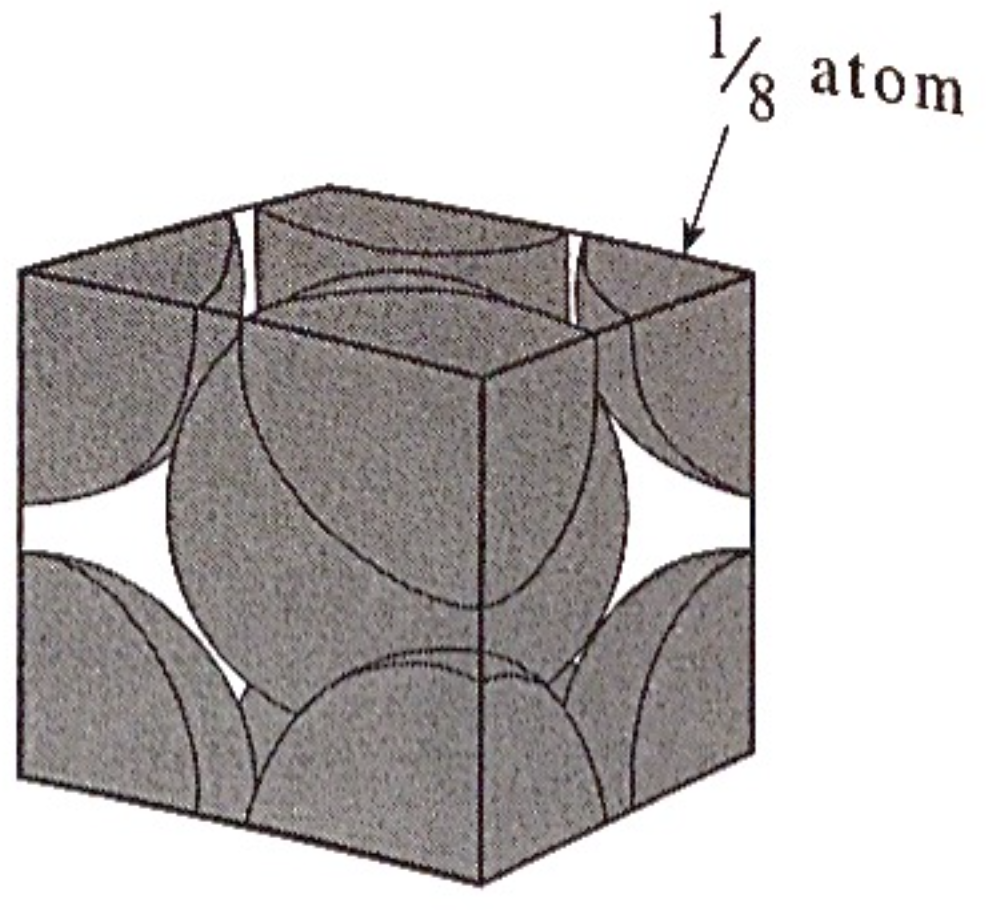
\includegraphics[width=0.85\linewidth]{../ExtFiles/BCCunitCellc.png}
            \caption{Unit cell.}
            \label{fig:BCCunitCellc}
        \end{subfigure}
        \caption{Body-centered cubic unit cell.}
        \label{fig:BCCunitCell}
    \end{figure}
    \begin{itemize}
        \item There are two atoms per unit cell.
        \item Example: The packing of potassium atoms in a crystal.
    \end{itemize}
    \item \textbf{Primitive cubic} (unit cell): The following unit cell. \emph{Also known as} \textbf{simple cubic}. \emph{Structure}
    \begin{figure}[h!]
        \centering
        \begin{subfigure}[b]{0.2\linewidth}
            \centering
            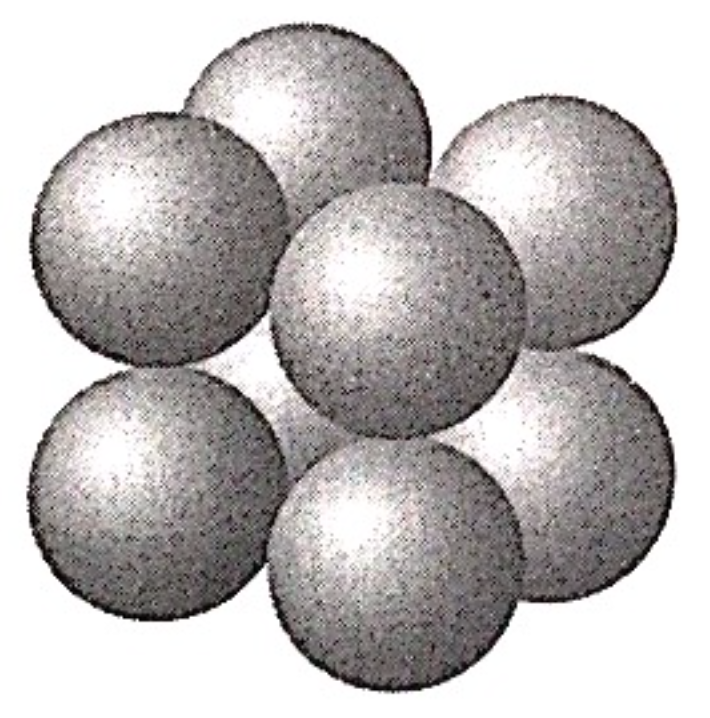
\includegraphics[width=0.6\linewidth]{../ExtFiles/PCunitCella.png}
            \caption{Atomic picture.}
            \label{fig:PCunitCella}
        \end{subfigure}
        \begin{subfigure}[b]{0.2\linewidth}
            \centering
            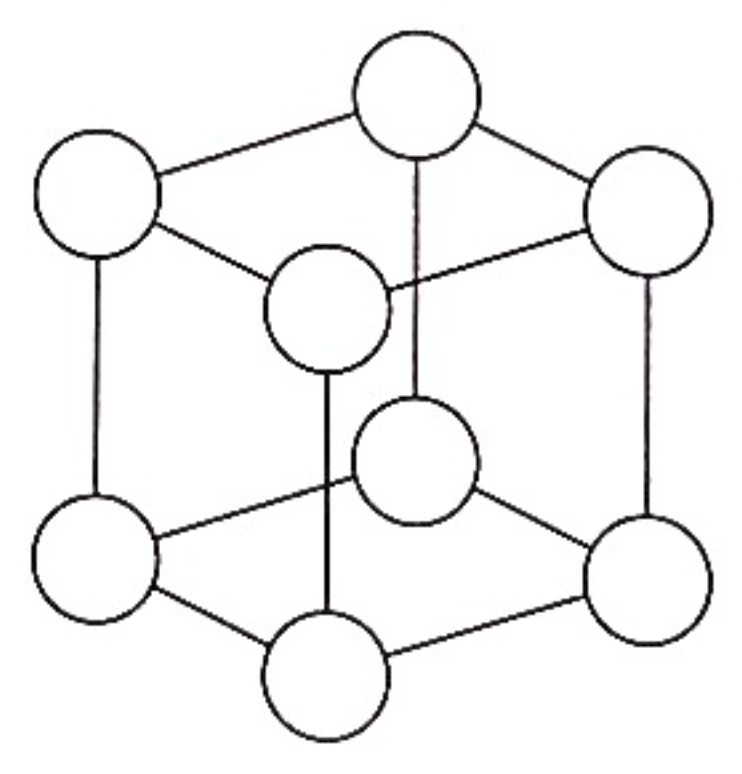
\includegraphics[width=0.65\linewidth]{../ExtFiles/PCunitCellb.png}
            \caption{Lattice picture.}
            \label{fig:PCunitCellb}
        \end{subfigure}
        \begin{subfigure}[b]{0.2\linewidth}
            \centering
            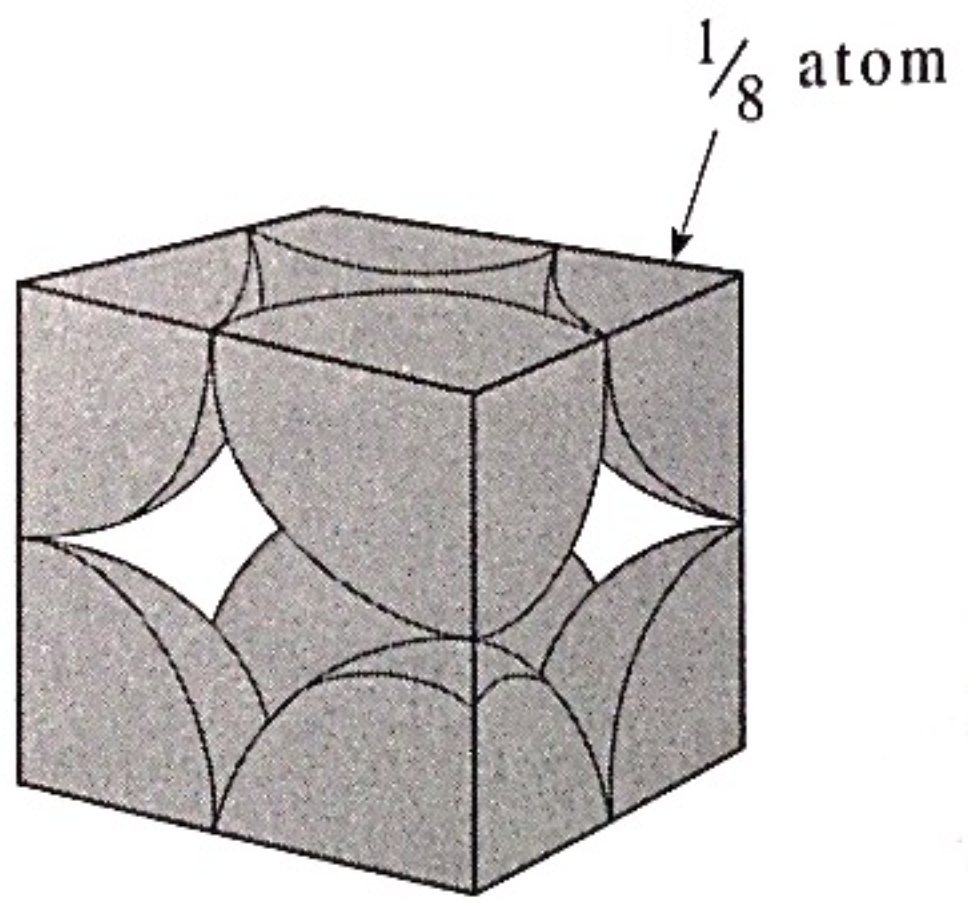
\includegraphics[width=0.85\linewidth]{../ExtFiles/PCunitCellc.png}
            \caption{Unit cell.}
            \label{fig:PCunitCellc}
        \end{subfigure}
        \caption{Body-centered cubic unit cell.}
        \label{fig:PCunitCell}
    \end{figure}
    \begin{itemize}
        \item There is one atom per unit cell.
        \item Example: The packing of polonium atoms in a crystal.
    \end{itemize}
    \item \textbf{Unit cell}: The simplest repeating unit in the crystal. \emph{Structure}
    \begin{figure}[H]
        \centering
        \begin{tikzpicture}[scale=2,z={(4.85mm,3.85mm)}]
            \footnotesize
            \draw
                (0,0,0) coordinate (O) -- node[below]{$a$} (1,0,0) coordinate (a) -- node[below right=-1pt]{$b$} (1,0,1) -- (0,0,1) coordinate (b) -- cycle
                (0.4,1.2,0) coordinate (c) -- ++(1,0,0) -- ++(0,0,1) -- ++(-1,0,0) -- cycle
                (O) -- (c)
                (a) -- ($(a)+(c)$)
                (b) -- ($(b)+(c)$)
                ($(a)+(b)$) -- node[right]{$c$} ($(a)+(b)+(c)$)
            ;
    
            \pic [draw,angle eccentricity=1.3,pic text={$\alpha$}] {angle=b--O--c};
            \pic [draw,angle radius=1cm] {angle=a--O--c};
            \node [fill=white,inner sep=1pt] at (20:0.5) {$\beta$};
            \pic [draw,angle radius=4mm,angle eccentricity=1.3,pic text={$\gamma$}] {angle=a--O--b};
    
            \draw [-stealth] ([xshift=-1cm]O) -- ([xshift=-1cm]$(O)!0.5!(a)$)  node[right]{\textbf{a}};
            \draw [-stealth] ([xshift=-1cm]O) -- ([xshift=-1cm]$(O)!0.65!(b)$) node[above right=-1pt]{\textbf{b}};
            \draw [-stealth] ([xshift=-1cm]O) -- ([xshift=-1cm]$(O)!0.5!(c)$)  node[right]{\textbf{c}};
        \end{tikzpicture}
        \caption{Unit cell.}
        \label{fig:unitCell}
    \end{figure}
    \begin{itemize}
        \item Opposite faces of a unit cell are parallel.
        \item The edge of the unit cell connects equivalent points.
        \item Unit cells all have the same general shape.
        \begin{itemize}
            \item We take the bottom left corner of the unit cell to be the origin of the \textbf{a}, \textbf{b}, \textbf{c} coordinate system.
            \item The unit cell is defined by the distances $a$, $b$, and $c$ (which give its length along the \textbf{a}, \textbf{b}, and \textbf{c} axes, respectively) and the angles $\alpha$, $\beta$, and $\gamma$ (which lie between the three pairs of axes).
        \end{itemize}
        \item Note that henceforth unless stated otherwise, the \textbf{a} axis points to the right, the \textbf{b} axis points back, and the \textbf{c} axis points up, as in Figure \ref{fig:unitCell}.
    \end{itemize}
    \item Tian gives examples of unit cells for crystals containing more than one atom as well as what kinds of crystals take these structures.
    \item \textbf{Bravais lattices}: The fourteen distinct unit cells necessary to generate all possible crystal lattices.
    \begin{itemize}
        \item The French physicist August Bravais proved that only the Bravais lattices are needed to generate all possible structures.
    \end{itemize}
    \item We can interpret the points in the unit cell as atoms or molecules. For example, crystalline \ce{C_{60}} forms a face-centered cubic unit cell.
    \item \textbf{Miller indices}: The three indices that we use to specify parallel planes through a crystal lattice. \emph{Denoted by} $\bm{h}$, $\bm{k}$, $\bm{l}$. \emph{Given by}
    \begin{align*}
        h &= \frac{a}{a'}&
        k &= \frac{b}{b'}&
        l &= \frac{c}{c'}
    \end{align*}
    where the plane in question intersects the \textbf{a}, \textbf{b}, and \textbf{c} axes of the unit cell at points $a'$, $b'$, and $c'$, respectively.
    \item Three basic types of planes.
    \begin{figure}[h!]
        \centering
        \begin{subfigure}[b]{0.2\linewidth}
            \centering
            \begin{tikzpicture}[z={(4.85mm,7mm)},line join=round]
                \draw [semithick] (0,0,0) -- (2,0,0) -- (2,0,1) -- (0,0,1) -- cycle;
                \filldraw [semithick,fill=rey]
                    (0,1,0) -- (0,0,0) -- (0,0,1) -- (0,1,1)
                    (1,1,0) -- (1,0,0) -- (1,0,1) -- (1,1,1)
                    (2,1,0) -- (2,0,0) -- (2,0,1) -- (2,1,1)
                ;
                \draw [semithick]
                    (0,1,0) -- (2,1,0) -- (2,1,1) -- (0,1,1) -- cycle
                    (1,1,0) -- (1,1,1)
                ;
            \end{tikzpicture}
            \caption{$100$ planes.}
            \label{fig:basicPlanesa}
        \end{subfigure}
        \begin{subfigure}[b]{0.2\linewidth}
            \centering
            \begin{tikzpicture}[z={(4.85mm,7mm)},line join=round]
                \draw [semithick] (0,0,0) -- (2,0,0) -- (2,0,1) -- (0,0,1) -- cycle;
                \draw [semithick]
                    (0,1,0) -- (0,0,0) -- (0,0,1) -- (0,1,1)
                    (1,1,0) -- (1,0,0) -- (1,0,1) -- (1,1,1)
                    (2,1,0) -- (2,0,0) -- (2,0,1) -- (2,1,1)
                ;
                \filldraw [semithick,fill=rey]
                    (1,0,0) -- (0,0,1) -- (0,1,1) -- (1,1,0) -- cycle
                    (2,0,0) -- (1,0,1) -- (1,1,1) -- (2,1,0) -- cycle
                ;
                \draw [semithick]
                    (0,1,0) -- (2,1,0) -- (2,1,1) -- (0,1,1) -- cycle
                    (1,1,0) -- (1,1,1)
                ;
            \end{tikzpicture}
            \caption{$110$ planes.}
            \label{fig:basicPlanesb}
        \end{subfigure}
        \begin{subfigure}[b]{0.2\linewidth}
            \centering
            \begin{tikzpicture}[z={(4.85mm,7mm)},line join=round]
                \draw [semithick] (0,0,0) -- (2,0,0) -- (2,0,1) -- (0,0,1) -- cycle;
                \draw [semithick]
                    (0,1,0) -- (0,0,0) -- (0,0,1) -- (0,1,1)
                    (1,1,0) -- (1,0,0) -- (1,0,1) -- (1,1,1)
                    (2,1,0) -- (2,0,0) -- (2,0,1) -- (2,1,1)
                ;
                \filldraw [semithick,fill=rey]
                    (1,0,0) -- (0,0,1) -- (0,1,0) -- cycle
                    (2,0,0) -- (1,0,1) -- (0,1,1) -- (1,1,0) -- cycle
                    (2,0,1) -- (2,1,0) -- (1,1,1) -- cycle
                ;
                \draw [semithick]
                    (0,1,0) -- (2,1,0) -- (2,1,1) -- (0,1,1) -- cycle
                    (1,1,0) -- (1,1,1)
                ;
            \end{tikzpicture}
            \caption{$111$ planes.}
            \label{fig:basicPlanesc}
        \end{subfigure}
        \caption{Basic lattice planes.}
        \label{fig:basicPlanes}
    \end{figure}
    \begin{itemize}
        \item Why are they called as such? Esp. where are the zeros coming from?
    \end{itemize}
    \item Denoting more complicated types of planes.
    \begin{figure}[H]
        \centering
        \begin{subfigure}[b]{0.2\linewidth}
            \centering
            \begin{tikzpicture}[z={(3.85mm,6mm)},line join=round,yscale=1.2]
                \path (0,0,0) -- (0,-1,0);
                \draw [semithick] (0,0,0) -- (1,0,0) -- (1,0,1) -- (0,0,1) -- cycle;
                \draw [semithick]
                    (0,1,0) -- (0,0,0) -- (0,0,1) -- (0,1,1)
                    (1,1,0) -- (1,0,0) -- (1,0,1) -- (1,1,1)
                ;
                \filldraw [semithick,fill=rey] (1,0,0.5) -- (0.5,0,1) -- (0.5,1,1) -- (1,1,0.5) -- cycle;
                \filldraw [semithick,fill=rey] (1,0,0) -- (0,0,1) -- (0,1,1) -- (1,1,0) -- cycle;
                \filldraw [semithick,fill=rex] (0.5,0,0) -- (0,0,0.5) -- (0,1,0.5) -- (0.5,1,0) -- cycle;
                \draw [semithick] (0,1,0) -- (1,1,0) -- (1,1,1) -- (0,1,1) -- cycle;
            \end{tikzpicture}
            \caption{$220$ planes.}
            \label{fig:complicatedPlanesa}
        \end{subfigure}
        \begin{subfigure}[b]{0.2\linewidth}
            \centering
            \begin{tikzpicture}[z={(3.85mm,6mm)},line join=round,yscale=1.2]
                \footnotesize
                \draw [semithick,dashed]
                    (0,0,1) -- (0,-1,1) -- (1,-1,1) -- (1,0,1)
                    (0,-1,1) -- (0,-1,0)
                    (1,-1,1) -- (1,-1,0)
                ;
                \filldraw [semithick,fill=rey] (1,-1,0) -- (1,0,1) -- (0,-1,1) -- cycle;
                \draw [semithick]
                    (0,1,1) -- (0,0,1) -- (1,0,1) -- (1,1,1)
                    (0,0,1) -- (0,0,0)
                    (1,0,1) -- (1,0,0)
                ;
                \filldraw [semithick,fill=rex] (0,-1,0) -- (1,0,0) -- (1,1,1) -- (0,0,1) -- cycle;
                \draw [semithick] (0,1,0) -- (0,1,1) -- (1,1,1) -- (1,1,0);
                \draw [semithick,dashed] (0,0,0) -- (0,-1,0) -- (1,-1,0) -- (1,0,0);
                \filldraw [semithick,fill=rey] (1,1,0) -- (0,1,1) -- (0,0,0) -- cycle;
                \draw [semithick] (0,1,0) -- (0,0,0) -- (1,0,0) -- (1,1,0) -- cycle;
    
                \node [left] at (0,1,0)  {$c$};
                \node [left] at (0,0,0)  {$0$};
                \node [left] at (0,-1,0) {$-c$};
            \end{tikzpicture}
            \caption{$11\bar{1}$ planes.}
            \label{fig:complicatedPlanesb}
        \end{subfigure}
        \caption{More complicated lattice planes.}
        \label{fig:complicatedPlanes}
    \end{figure}
    \begin{itemize}
        \item In Figure \ref{fig:complicatedPlanesa}, we denote by $220$ the darkened plane and implicitly identify planes that are stacked twice as close together as in Figure \ref{fig:basicPlanesb}.
        \begin{itemize}
            \item Note that $h=a/a'=a/(a/2)=2$ and $k=b/b'=b/(b/2)$ is where the twos are coming from.
        \end{itemize}
        \item In Figure \ref{fig:complicatedPlanesb}, we denote by $11\bar{1}$ the darkened plane. The $\bar{1}$ denotes a Miller index of \emph{negative} one, corresponding to $c'=-c$ (notice how the darkened plane does not intersect the \textbf{c} axis within the unit cell, but rather extends down to the axis' negative region).
    \end{itemize}
    \item The lattice plane spacing can be determined.
    \begin{itemize}
        \item The perpendicular distance between adjacent $hkl$ planes for an orthorhombic unit cell.
        \begin{equation*}
            \frac{1}{d^2} = \frac{h^2}{a^2}+\frac{k^2}{b^2}+\frac{l^2}{c^2}
        \end{equation*}
        \item For a cubic unit cell,
        \begin{equation*}
            \frac{1}{d^2} = \frac{h^2+k^2+l^2}{a^2}
        \end{equation*}
        \item For a tetragonal unit cell,
        \begin{equation*}
            \frac{1}{d^2} = \frac{h^2+k^2}{a^2}+\frac{l^2}{c^2}
        \end{equation*}
        \item For a hexagonal unit cell,
        \begin{equation*}
            \frac{1}{d^2} = \frac{4}{3}\left( \frac{h^2+hk+k^2}{a^2} \right)+\frac{l^2}{c^2}
        \end{equation*}
        \item For a rhombohedral unit cell,
        \begin{equation*}
            \frac{1}{d^2} = \frac{(h^2+k^2+l^2)\sin^2\alpha+2(hk+kl+hl)(\cos^2\alpha-\cos\alpha)}{a^2(1-3\cos^2\alpha+2\cos^3\alpha)}
        \end{equation*}
        \item For a monoclinic unit cell,
        \begin{equation*}
            \frac{1}{d^2} = \frac{1}{\sin^2\beta}\left( \frac{h^2}{a^2}+\frac{k^2\sin^2\beta}{b^2}+\frac{l^2}{c^2}-\frac{2hl\cos\beta}{ac} \right)
        \end{equation*}
        \item For a triclinic unit cell,
        \begin{equation*}
            \frac{1}{d^2} = \frac{1}{V^2}(S_{11}h^2+S_{22}k^2+S_{33}l^2+2S_{12}hk+2S_{23}kl+2S_{13}hl)
        \end{equation*}
        where
        \begin{align*}
            S_{11} &= b^2c^2\sin^2\alpha&
                S_{12} &= abc^2(\cos\alpha\cos\beta-\cos\gamma)\\
            S_{22} &= a^2c^2\sin^2\beta&
                S_{23} &= a^2bc(\cos\beta\cos\gamma-\cos\alpha)\\
            S_{33} &= a^2b^2\sin^2\gamma&
                S_{13} &= ab^2c(\cos\gamma\cos\alpha-\cos\beta)\\
        \end{align*}
    \end{itemize}
\end{itemize}



\section{Chapter 30: Gas-Phase Reaction Dynamics}
\emph{From \textcite{bib:McQuarrieSimon}.}
\begin{itemize}
    \item \marginnote{5/21:}We will now build a molecular picture of the \ce{F + D2} chemical reaction from the crossed molecular beam data. We take $E_\text{react}=\SI{7.62}{\kilo\joule\per\mole}$ throughout the following, as per the previous example.
    \item The \emph{angle} with which the molecules reach the detector.
    \begin{itemize}
        \item As per Figure \ref{fig:COMcoordinates} and the associated discussion, $\mathbf{u}_{\ce{DF}}'$ and $\mathbf{u}_{\ce{D}}'$ are not independent but are related by the conservation laws for mass, momentum, and energy.
        \item However, even though this means that \ce{DF} and \ce{D} could theoretically part ways in any manner consistent with these three laws, in reality, they will go their separate ways in some directions far more often than others, as dictated by the dynamics of this particular reaction.
        \item Let's consider these dynamics in greater detail, as facilitated by Figure \ref{fig:velocityAngleDist}.
        \begin{itemize}
            \item In this picture, we take as our reference frame the perspective of spherically symmetric molecule \ce{B} and let \ce{A} approach.
            \item For $b$ fixed, the distribution in $\phi$ will be cylindrically symmetric.
            \item \marginnote{5/22:}However, the angle $\theta$ will vary.
        \end{itemize}
    \end{itemize}
    \item The \emph{speed} at which the molecules hit the detector.
    \begin{figure}[h!]
        \centering
        \begin{tikzpicture}[xscale=0.9]
            \small
            \draw (-1,3) -- node[rotate=90,above,align=center]{Number of\\molecules detected} (-1,0) -- node[below]{$t$} (5,0);
            \footnotesize
            \node at (0,2.5) {$v=0$};
            \node at (1,2.5) {$1$};
            \node at (2,2.5) {$2$};
            \node at (3,2.5) {$3$};
            \node at (4,2.5) {$4$};
    
            \draw [blx,thick] (-1,0.3)
                -- (0.5,0.3)
                to[out=0,in=180] (1,0.4)
                to[out=0,in=180] (1.5,0.3)
                to[out=0,in=180,out looseness=0.7,in looseness=0.4] (2,1.2)
                to[out=0,in=180,out looseness=0.4,in looseness=0.7] (2.5,0.3)
                to[out=0,in=180,out looseness=0.5,in looseness=0.2] (3,2.2)
                to[out=0,in=180,out looseness=0.2,in looseness=0.5] (3.5,0.3)
                to[out=0,in=180,out looseness=0.7,in looseness=0.4] (4,1.3)
                to[out=0,in=180,out looseness=0.4,in looseness=0.7] (4.5,0.3)
                to (5,0.3)
            ;
        \end{tikzpicture}
        \caption{\ce{DF} speed distribution.}
        \label{fig:DFspeeds}
    \end{figure}
    \begin{itemize}
        \item Additionally, as per the previous example, \ce{DF} can be produced in vibrational states zero through four.
        \item \textcite{bib:McQuarrieSimon} does a worked example, showing quantitatively how the speed of the \ce{DF} molecule depends on its vibrational state.
        \item Experimentally, these results show up as separate peaks, each corresponding to a vibrational energy level, in Figure \ref{fig:DFspeeds}, which gives the collision frequency of \ce{DF} molecules with the detector over time.
        \begin{itemize}
            \item Notice that the molecules with the least vibrational energy have the most translational energy, and hence move the fastest and appear first.
        \end{itemize}
    \end{itemize}
    \item \marginnote{5/24:}We represent the distribution in angle and speed for a given reaction all at once with a 2D polar contour plot.
    \begin{figure}[h!]
        \centering
        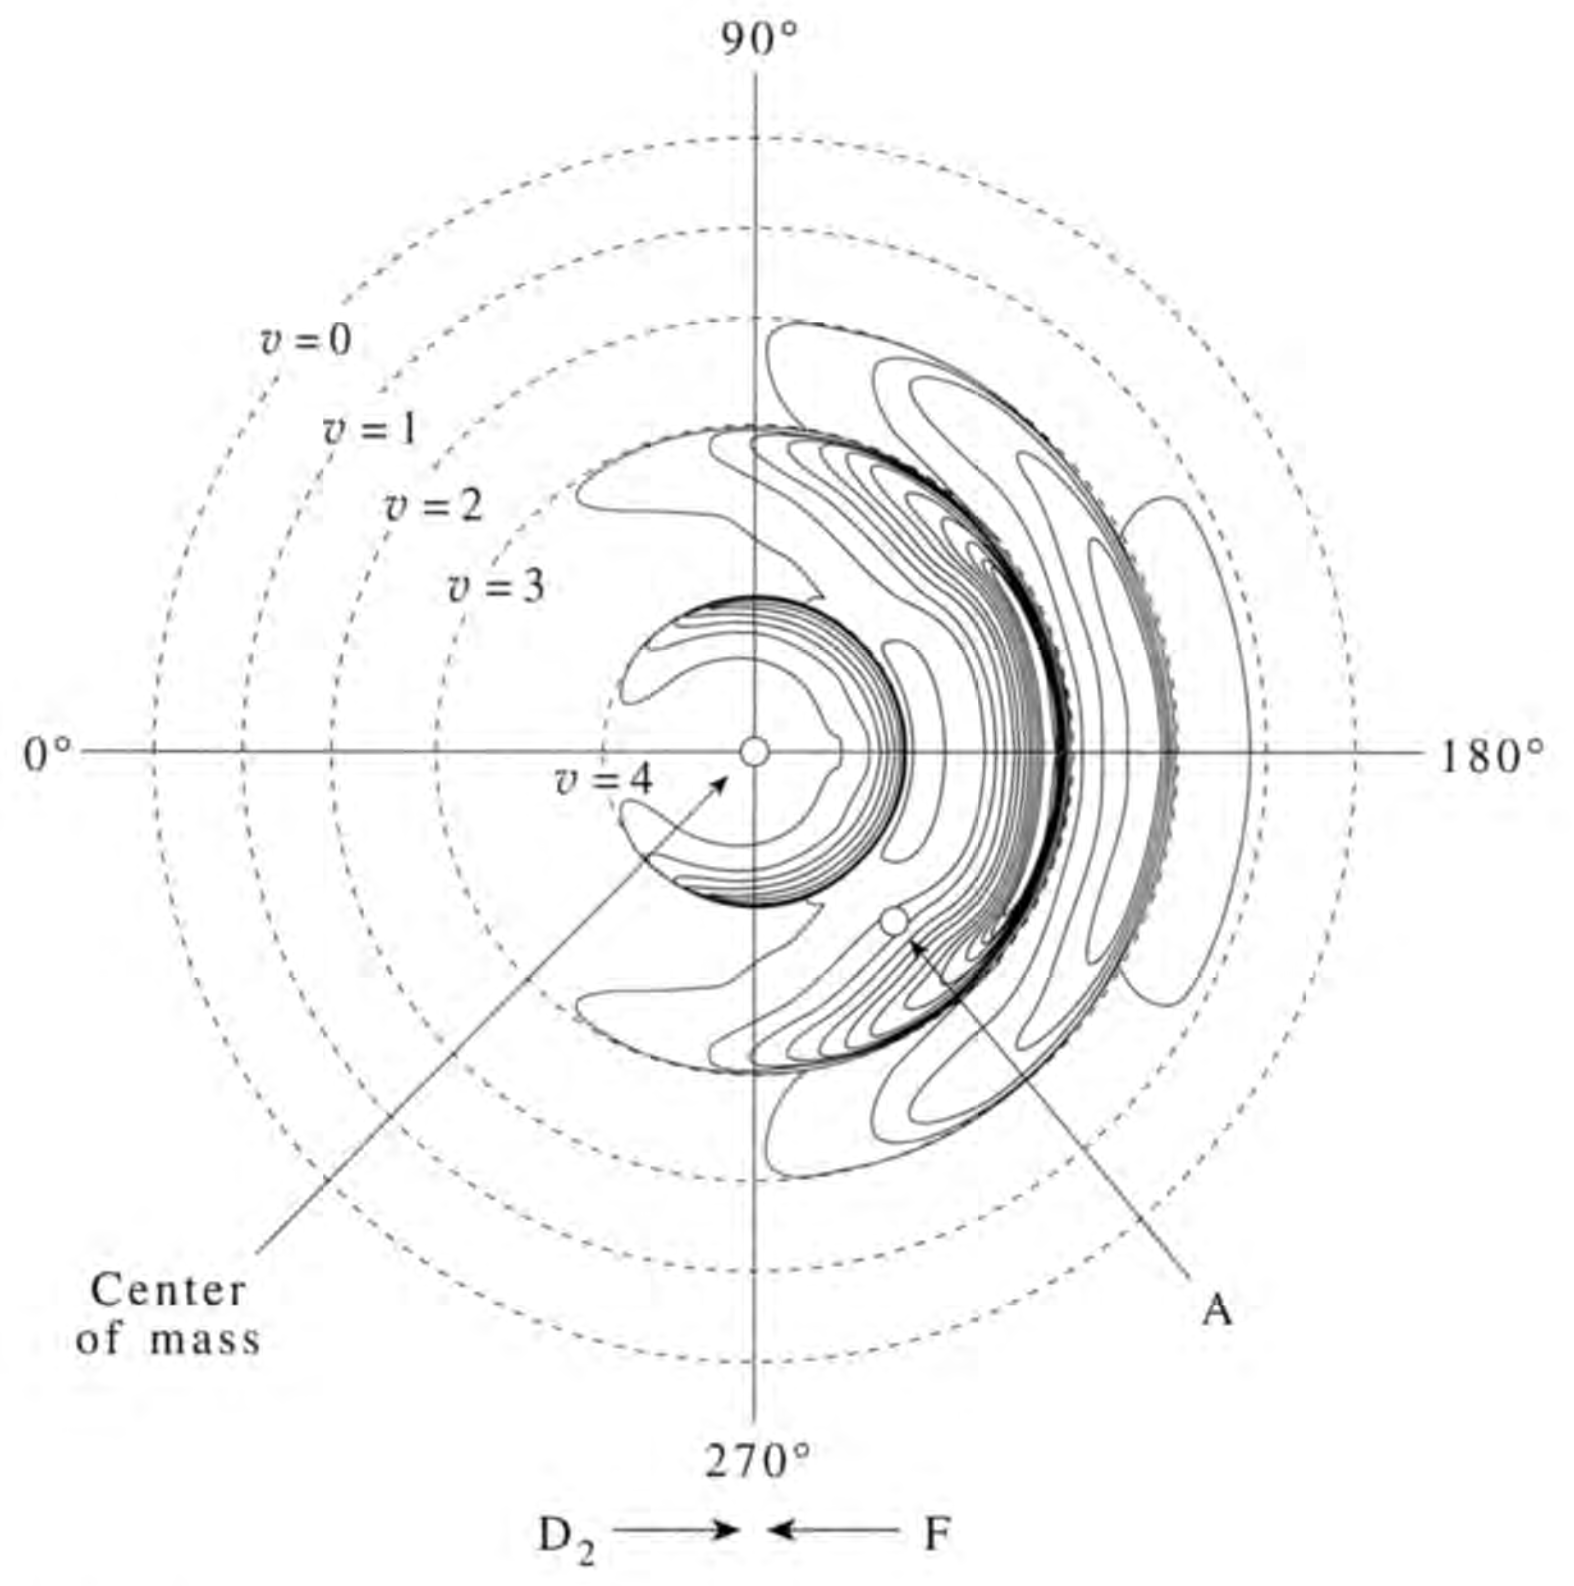
\includegraphics[width=0.53\linewidth]{../ExtFiles/ContourPlotFD2.png}
        \caption{Contour plot for \ce{F + D2}.}
        \label{fig:ContourPlotFD2}
    \end{figure}
    \begin{itemize}
        % \item This plot describes the angular distribution of \ce{DF} molecules after they leave the reaction site.
        \item The center of mass (see Figure \ref{fig:COMcoordinates}) sits at the center of the contour plot.
        % \item The distance from the origin to any point gives the speed $|\mathbf{u}_{\ce{DF}}-\mathbf{u}_\text{cm}|$ relative to the center of mass of a particular \ce{DF} molecule, i.e., points farther from the center account for molecules that traveled to the detector faster.
        \item The arrows below the plot indicate the directions with which the reactants approached each other relative to the center of mass. In other words, the horizontal axis lies along the relative velocity vector of the reactants (see Figure \ref{fig:COMcoordinates}).
        \item The indicated angles correspond to the \textbf{scattering angle} $\theta$ (which is the complement of the angle $\theta$ from Figure \ref{fig:velocityAngleDist}).
        \item The contour lines represent a constant number of \ce{DF} molecules.
        \item The dashed lines represent the maximum relative speed allowed for a \ce{DF} molecule in a given vibrational state.
        \begin{itemize}
            \item An increase in diameter corresponds to greater speed and lower vibration.
            \item Note that all circles drawn correspond to rotational energy $E_\text{rot}=0$ with $J=0$. If a molecule is produced in a rotationally excited state, it must have a slower speed than the maximum allowed by its vibrational state. Consider a molecule located at position A in the diagram, for instance --- for the molecule to have such a speed, it must either be rotationally excited, or have had more of the energy in its collision go into the translational energy of the other product (\ce{D}).
        \end{itemize}
        % \item Notice that the contour density is greatest between vibrational states $v=3$ and $v=4$ (i.e., with molecules that have $v=3$) and that there is no contour density between vibrational states $v=0$ and $v=1$ (i.e., with molecules that have $v=0$), in agreement with Figure \ref{fig:DFspeeds}.
    \end{itemize}
    \item \textbf{Scattering angle} (in an atom-molecule reaction): The angle between the relative velocity vector of the atomic reactant and the relative velocity vector of the product containing the formerly lone atom. \emph{Denoted by} $\bm{\theta}$.
    \begin{itemize}
        \item In \ce{F + D2}, the scattering angle is the change in the direction of the \ce{F}-containing species. Indeed, since \ce{DF} leaves the collision region in the same direction in which \ce{F} entered in general, $\theta\approx\ang{180}$ in general for \ce{F + D2}, as is readily read from Figure \ref{fig:ContourPlotFD2}.
    \end{itemize}
    \item Further considerations of the scattering angle.
    \begin{figure}[h!]
        \centering
        \begin{subfigure}[b]{0.25\linewidth}
            \centering
            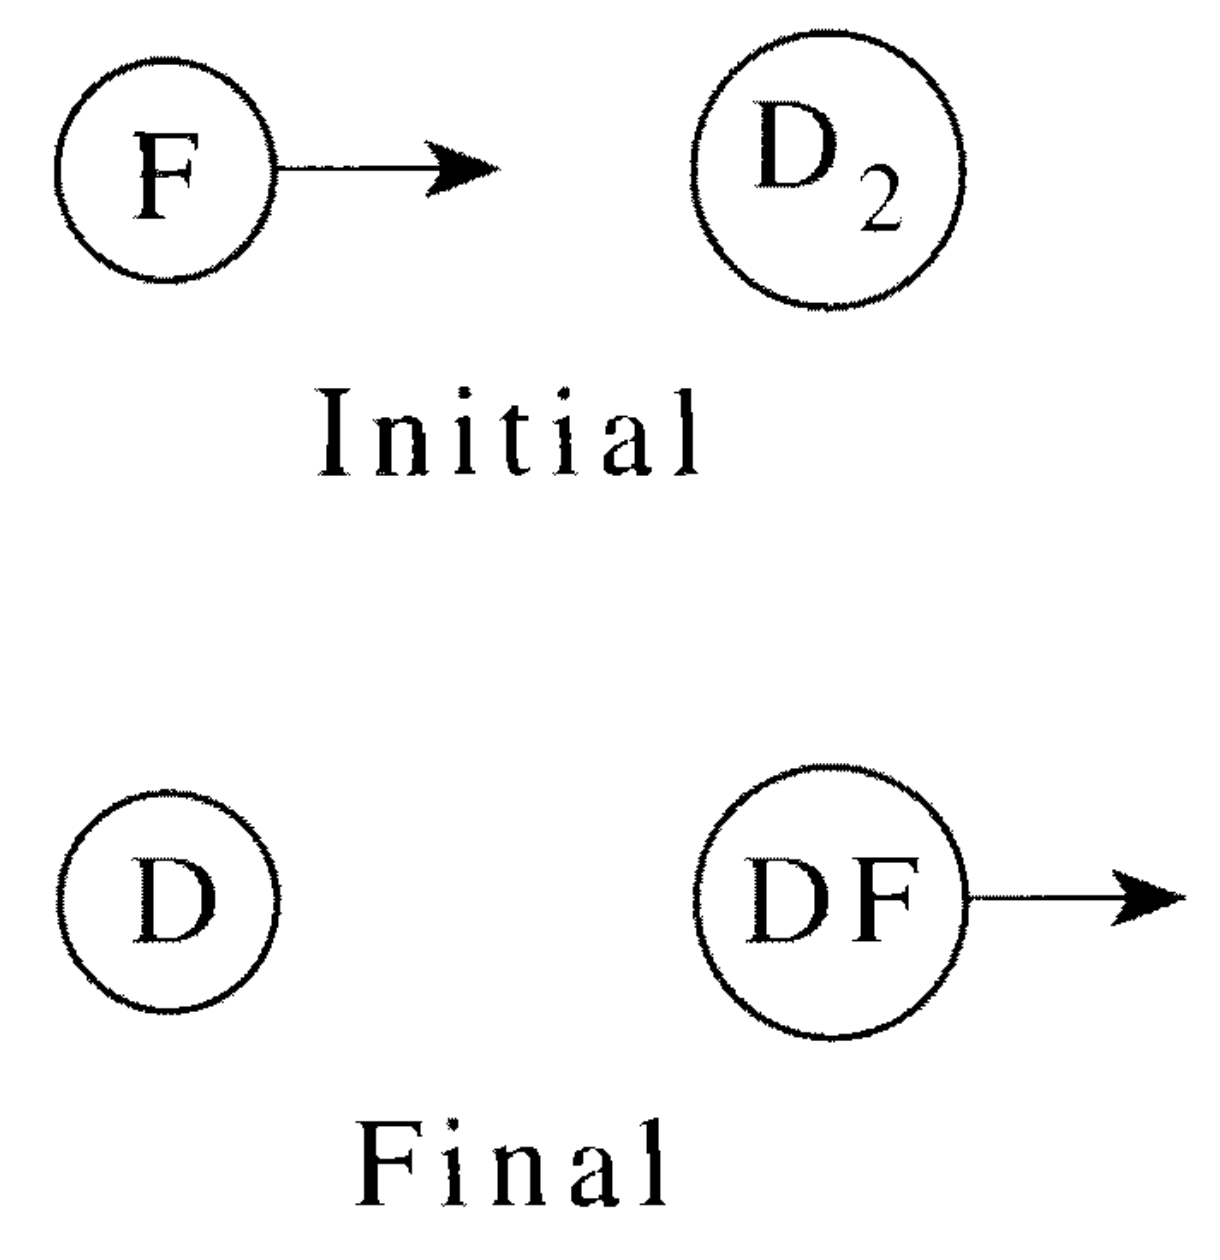
\includegraphics[width=0.7\linewidth]{../ExtFiles/FD2scatteringa.png}
            \caption{$\theta=\ang{0}$}
            \label{fig:FD2scatteringa}
        \end{subfigure}
        \begin{subfigure}[b]{0.25\linewidth}
            \centering
            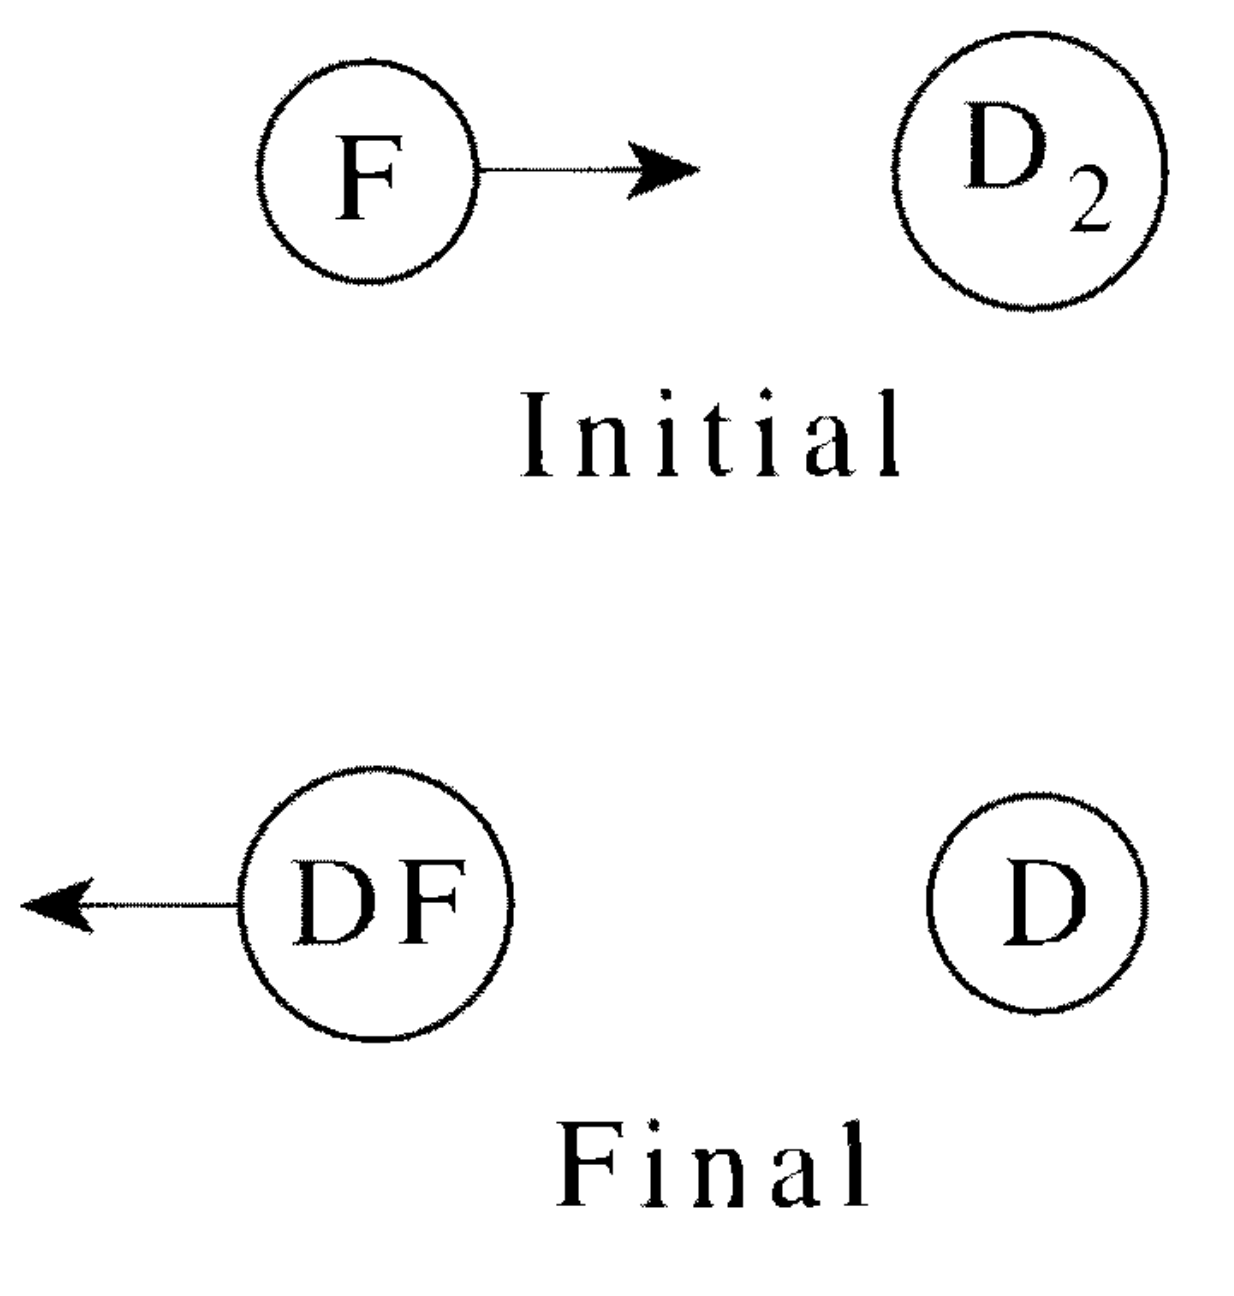
\includegraphics[width=0.7\linewidth]{../ExtFiles/FD2scatteringb.png}
            \caption{$\theta=\ang{180}$}
            \label{fig:FD2scatteringb}
        \end{subfigure}
        \caption{Scattering angles in the atom-molecule reaction \ce{F + D2}.}
        \label{fig:FD2scattering}
    \end{figure}
    \begin{itemize}
        \item Figure \ref{fig:FD2scattering} shows the cases of $\theta=\ang{0}$ and $\theta=\ang{180}$ for \ce{F + D2}.
        \item Thus, the fact that \ce{DF} preferentially scatters with $\theta\approx\ang{180}$ tells us that, in terms of Figure \ref{fig:COMcoordinates}, we may have $\ce{A}=\ce{F}$ and $\ce{C}=\ce{DF}$ or vice versa so that the direction at which fluorine enters is the direction at which \ce{DF} leaves; importantly, we do \emph{not} have a case of $\ce{A}=\ce{F}$ and $\ce{D}=\ce{DF}$, in which the \ce{F}-containing product leaves in the same relative direction at which the \ce{F}-containing reactant entered.
        \item "In an atom-molecule reaction, we take $\theta=\ang{0}$ to lie along the direction defined by the trajectory of the incident atom" \parencite[1252]{bib:McQuarrieSimon}.
        % \item Additionally (although this picture can be more confusing than helpful here), we can discuss the collision in terms of Figure \ref{fig:velocityAngleDist}. Here, we have molecule $\ce{B}=\ce{F}$ and $\ce{A}=\ce{D2}$ so that the blue sphere on the right is \ce{DF} (\ce{D} is not shown here, but it would bounce back in the direction of \ce{A}/\ce{D2}).
    \end{itemize}
    \item Relating Figure \ref{fig:ContourPlotFD2} to the crossed molecular beam experimental setup in Figure \ref{fig:crossedMolBeama}.
    \begin{itemize}
        \item In looking at Figure \ref{fig:ContourPlotFD2}, imagine that we are located between the two molecular beam sources in Figure \ref{fig:crossedMolBeama} and looking at the collision region. Let the blue molecules be \ce{D2} and the red atoms be \ce{F} (from our vantage point, this would make it look like \ce{F} is coming in from the right and \ce{D2} from the left, as in Figure \ref{fig:ContourPlotFD2}). Additionally, the center of mass would not appear to be moving from our perspective because it would be moving away from us.
        \item When two molecules collide, we would see (from our vantage point) molecules of \ce{DF} exiting the collision region to the right more often than to the left; these molecules account for the preferential \ang{180} scattering observed in Figure \ref{fig:ContourPlotFD2}.
    \end{itemize}
    \item Example: Determining the rotational state of point A in Figure \ref{fig:ContourPlotFD2}.
    \begin{itemize}
        \item It is determined that the \ce{DF} molecule at point A has total rovibrational energy \SI{11493.6}{\per\centi\meter} and vibrational quantum number $v=3$. Additionally, we find that
        \begin{center}
            \small
            \renewcommand{\arraystretch}{1.2}
            \begin{tabular}{cccc}
                $\tilde{\nu}_e$ (\si{\per\centi\meter}) & $\tilde{\nu}_e\tilde{x}_e$ (\si{\per\centi\meter}) & $\tilde{B}_e$ (\si{\per\centi\meter}) & $\tilde{\alpha}_e$ (\si{\per\centi\meter})\\
                \hline
                \num{2998.3} & \num{45.71} & \num{11.007} & \num{0.293}\\
            \end{tabular}
        \end{center}
        \item From Chapter 13 and the above data, we have that
        \begin{align*}
            E_\text{vib}(v) &= \tilde{\nu}_e\left( v+\tfrac{1}{2} \right)-\tilde{\nu}_e\tilde{x}_e\left( v+\tfrac{1}{2} \right)^2&
                E_\text{rot}(J,v) &= \left[ \tilde{B}_e-\tilde{\alpha}_e\left( v+\tfrac{1}{2} \right) \right]J(J+1)\\
            &= \SI{9934.1}{\per\centi\meter}&
                &= (\SI{9.982}{\per\centi\meter})J(J+1)
        \end{align*}
        \item Therefore,
        \begin{align*}
            E_\text{tot}(J,v) &= E_\text{vib}(v)+E_\text{rot}(J,v)\\
            \SI{11493.6}{\per\centi\meter} &= \SI{9934.1}{\per\centi\meter}+(\SI{9.982}{\per\centi\meter})J(J+1)\\
            J(J+1) &= 156\\
            J &= 12
        \end{align*}
        as desired.
    \end{itemize}
    \item Three important features of the \ce{F + D2} reaction, as determined from Figure \ref{fig:ContourPlotFD2}.
    \begin{enumerate}
        \item The reaction is a \textbf{rebound reaction}.
        \item The most probable product of the reaction is $\ce{DF}(v=3)$.
        \item There is considerable population between the dashed circles, indicating that \ce{DF} molecules are produced in a variety of rotational levels.
    \end{enumerate}
    \item \textbf{Rebound reaction}: An atom-molecule reaction in which the atom undergoes a nearly head-on collision with the molecule and then bounces backward after abstracting one of the atoms from the molecule.
    \item Notice that the vibrational levels are populated in a distribution consistent with Figure \ref{fig:DFspeeds}, not the M-B distribution.
    \begin{itemize}
        \item This is called a \textbf{nonequilibrium product distribution}.
        \item We can use the Boltzmann factor to calculate the distribution in \ce{DF} vibrational states at thermal equilibrium as follows.
        \begin{equation*}
            \frac{N(v)}{N(3)} = \frac{\e[-(v+1/2)h\nu_{\ce{DF}}/\kB T]}{\e[-(3+1/2)h\nu_{\ce{DF}}/\kB T]}
            = \e[-(v-3)h\nu_{\ce{DF}}/\kB T]
        \end{equation*}
        \item This reveals that the vibrational state $v$ should be approximately $6(3-v)$ orders of magnitude more populated than $v=3$ at \SI{300}{\kelvin}. In particular, $v=0$ should be approximately 18 orders of magnitude more populated than $v=3$ at said temperature, $v=1$ should be approximately 12 orders of magnitude more populated than $v=3$, and so on and so forth.
    \end{itemize}
    \item \textbf{Stripping reaction}: An atom-molecule reaction in which the incident atom abstracts part of a molecule and keeps going in the forward direction.
    \item \textbf{Harpoon mechanism}: The mechanism by which a stripping reaction occurs, involving the formation of ions, followed by Coulombic attraction, followed by a reaction.
    \begin{itemize}
        \item So named because the species which becomes a cation uses its electron as a "harpoon" to draw in (via the Coulomb potential) the species which becomes an anion.
    \end{itemize}
    \item Evidence for the harpoon mechanism.
    \begin{itemize}
        \item Consider the stripping reaction
        \begin{equation*}
            \ce{K(g) + I2(g) -> KI(g) + I(g)}
        \end{equation*}
        in which the relative translational energy between the reactants is $E_\text{trans}=\SI{15.13}{\kilo\joule\per\mole}$.
        \item The contour plot shows a primary scattering angle of $\theta\approx\ang{0}$.
        \begin{itemize}
            \item Thus, it would appear that electric fields are not repulsing the molecules as we would expect in a head-on collision.
        \end{itemize}
        \item The reaction cross section is twice the collision cross section.
        \begin{itemize}
            \item We can measure the reaction cross section of \ce{K + I2} to be \SI{1.25e6}{\pico\meter\squared}.
            \item Based on the measured radii of \ce{K} and \ce{I2} as \SI{205}{\pico\meter} and \SI{250}{\pico\meter}, respectively, we have that $\sigma_{\ce{K}\ \ce{I2}}=\SI{6.5e5}{\pico\meter\squared}$.
            \item Indeed, this means that if the reactants travel at the maximum impact parameter (see Figure \ref{fig:lineOfCenters}), they would miss each other entirely but somehow still react.
        \end{itemize}
        \item An electron transfer occurs between the two reactants before they collide.
        \begin{itemize}
            \item If two molecules are to react without touching, they must somehow be attracted to each other in manner strong enough to at least temporarily overcome the bond-dissociation energy (BDE) of the molecule.
            \item Research shows that van der Waals interactions would not be strong enough for this, but a Coulomb potential would be.
            \item Additionally, we can directly experimentally verify that this pre-reaction electron transfer occurs.
        \end{itemize}
    \end{itemize}
    \item Reactions in which the scattering angle is fairly equally distributed.
    \begin{itemize}
        \item This cannot be either a hit-and-run collision or a drive-by collision.
        \item Indeed, the only explanation is that lifetime of the atom-molecule complex is long compared with the rotation period, so that the reactants "forget" their initial orientation while reacting and then break apart in relatively random directions.
        \item An example reaction that proceeds in this fashion is
        \begin{equation*}
            \ce{O(g) + Br2(g)} \Longrightarrow \ce{BrO(g) + Br(g)}
        \end{equation*}
    \end{itemize}
    \item \textcite{bib:McQuarrieSimon} discusses the three variables that determine the potential energy surface of a water molecule and the analogous three variables that determine the potential energy surface of \ce{F + D2}.
    \item We can't represent these potential energy surfaces with a 2D- or 3D graph (we'd need four axes), so we have to turn to cross sections (i.e., fixing one of the variables and plotting the other two).
    \item The potential energy surface for a reaction can be computed using the electronic structure techniques of Chapter 11.
    \item \textbf{Collinear geometry}: A reactive collision with $\beta=\ang{180}$ (see Figure \ref{fig:FD2attackAnglea}).
    \item The potential energy surface for \ce{F + D2} in a collinear geometry.
    \begin{figure}[H]
        \centering
        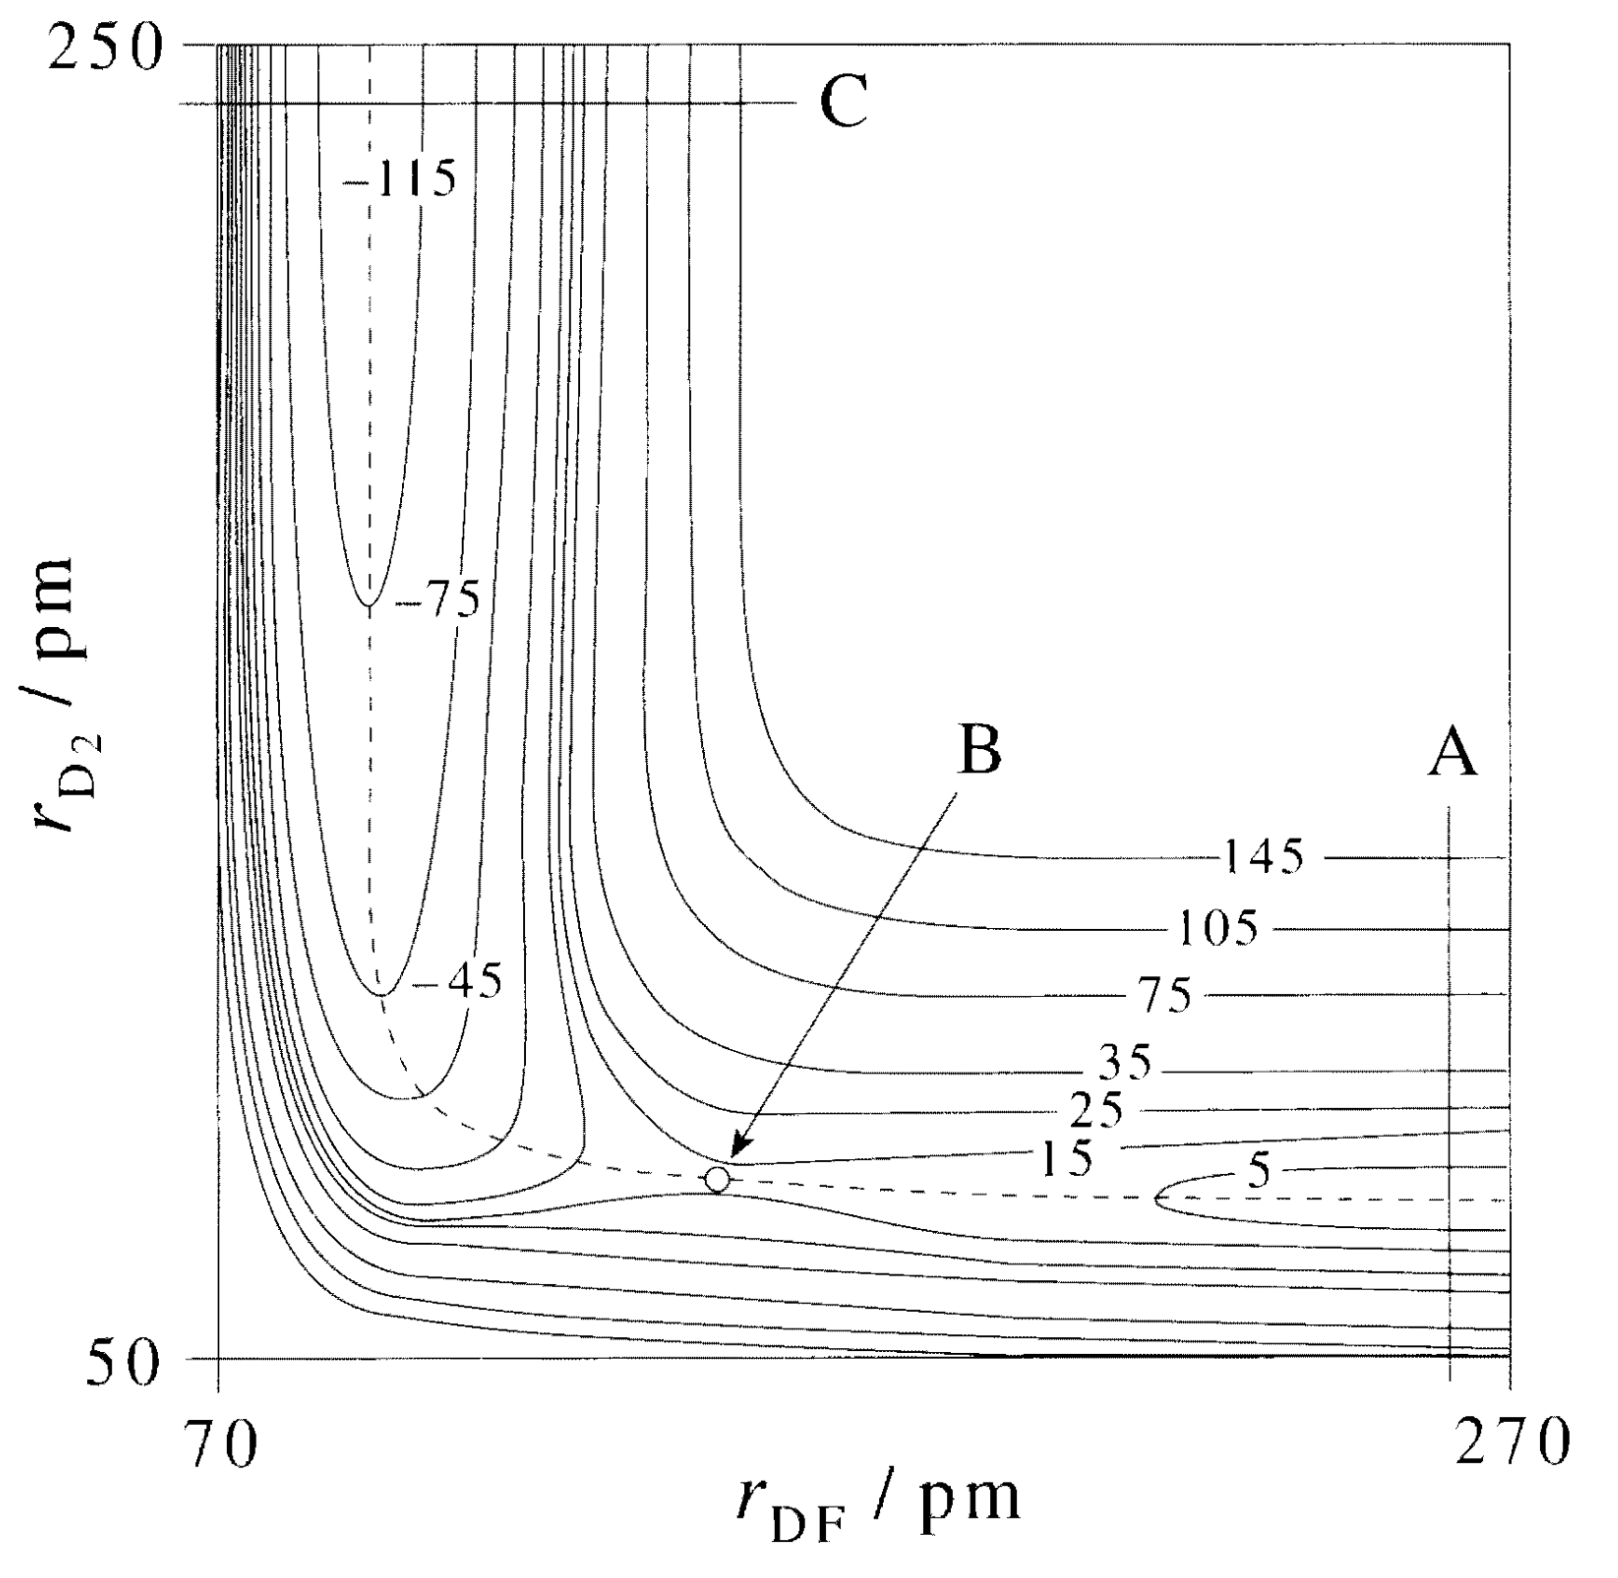
\includegraphics[width=0.4\linewidth]{../ExtFiles/FD2PEScollinear.png}
        \caption{The potential energy surface for \ce{F + D2} where $\beta=\ang{180}$.}
        \label{fig:FD2PEScollinear}
    \end{figure}
    \begin{itemize}
        \item Each line in the contour map corresponds to a constant value of energy.
        \item The numbers on the lines express the energy of that line in \si{\kilo\joule\per\mole}.
        \item The zero of energy is taken to be the infinitely separated reactants.
        \item The cross section of the contour plot at A gives the potential energy curve for \ce{D2}.
        \item The cross section of the contour plot at C gives the potential energy curve for \ce{DF}.
        \item The dashed line proceeds from the bottom right to the top left and traces the reaction coordinate along the lowest-energy path.
        \item Point B indicates the transition state.
        \item Notice how as we trace the progress of the reaction, we start at energy near zero, climb the activation energy hill (passing the \SI{5}{\kilo\joule\per\mole} contour but not quite reaching the \SI{15}{\kilo\joule\per\mole} contour; the true value of the activation energy is approximately \SI{7}{\kilo\joule\per\mole}), pass the transition state at a \textbf{saddle point}, and rapidly decrease in energy thereafter (this is an exergonic reaction).
        \item This diagram also gives meaning to the principle of microscopic reversibility, i.e., that a reaction (forwards or backwards) will always follow the lowest energy path.
    \end{itemize}
\end{itemize}



\section{Chapter 31: Solids and Surface Chemistry}
\emph{From \textcite{bib:McQuarrieSimon}.}
\begin{itemize}
    \item Goals of the chapter.
    \begin{itemize}
        \item Solid-state chemistry: Crystal structure and how X-ray diffraction can be used to determine it.
        \item \textbf{Surface chemistry}.
        \item Nitrogen fixation on iron catalysts.
    \end{itemize}
    \item \textbf{Surface chemistry}: The study of how the surfaces of solids catalyze chemical reactions.
    \item Looking at a crystal reveals a periodic structure that we should be able to take advantage of to describe its structure in general. To this effect, we define the \textbf{unit cell}.
    \item \textbf{Unit cell}: The smallest collection of atoms (or molecules) in the crystal such that the replication of the unit cell in three dimensions generates the entire crystal.
    \item A unit cell cannot have any arbitrary shape.
    \begin{itemize}
        \item A spherical unit cell would leave gaps, for instance.
        \item It is also impossible to generate a crystal lattice by a unit cell that has a five-fold symmetry axis (see Problem \ref{prb:31-43}).
        \item Indeed, "the unit cell must be a geometric structure that fills all space when replicated" \parencite[1272]{bib:McQuarrieSimon}.
    \end{itemize}
    \item \textcite{bib:McQuarrieSimon} defines \textbf{face-centered cubic}, \textbf{body-centered cubic}, and \textbf{primitive cubic} unit cells.
    \item These are the only three types of cubic unit cells!
    \item \textcite{bib:McQuarrieSimon} develops a method of describing the most general type of unit cell (a three-dimensional parallelepiped) as in lecture (see the discussion associated with Figure \ref{fig:unitCell}).
    \item \textcite{bib:McQuarrieSimon} defines the \textbf{Bravais lattices}.
    \begin{table}[H]
        \centering
        \small
        \renewcommand{\arraystretch}{1.4}
        \begin{tabular}{cccccc}
             & P & I & C & F & R\\
            \begin{tabular}{@{}c@{}}
                Triclinic\\[-2mm]
                \footnotesize
                $a\neq b\neq c$\\[-2mm]
                \footnotesize
                $\alpha\neq\beta\neq\gamma$
            \end{tabular}
                & \tikz[baseline={(0,0.6)},scale=0.7]{
                    \path (0,-0.4) -- (0,2.3);
                    \filldraw [fill=white]
                        (0,0) coordinate (O) circle (1.5pt)
                        (1.38,0) coordinate (a) circle (1.5pt)
                        (0.64,0.26) coordinate (b) circle (1.5pt)
                        (-0.22,1.6) coordinate (c) circle (1.5pt)
                        ($(a)+(b)$) coordinate (ab) circle (1.5pt)
                        ($(a)+(c)$) coordinate (ac) circle (1.5pt)
                        ($(b)+(c)$) coordinate (bc) circle (1.5pt)
                        ($(a)+(b)+(c)$) coordinate (abc) circle (1.5pt)
                    ;
                    \begin{scope}[on background layer]
                        \draw [line join=bevel]
                            (O) -- (a) -- (ab) -- (b) -- cycle
                            (c) -- (ac) -- (abc) -- (bc) -- cycle
                            (O) -- (c)
                            (a) -- (ac)
                            (b) -- (bc)
                            (ab) -- (abc)
                        ;
                    \end{scope}
                }
                &  &  &  & \\
            \begin{tabular}{@{}c@{}}
                Monoclinic\\[-2mm]
                \footnotesize
                $a\neq b\neq c$\\[-2mm]
                \footnotesize
                $\gamma\neq\alpha=\beta=\ang{90}$
            \end{tabular}
                & \tikz[baseline={(0,0.6)},scale=0.7]{
                    \path (0,-0.4) -- (0,2.3);
                    \filldraw [fill=white]
                        (0,0) coordinate (O) circle (1.5pt)
                        (1.3,0) coordinate (a) circle (1.5pt)
                        (0.62,0.24) coordinate (b) circle (1.5pt)
                        (0,1.65) coordinate (c) circle (1.5pt)
                        ($(a)+(b)$) coordinate (ab) circle (1.5pt)
                        ($(a)+(c)$) coordinate (ac) circle (1.5pt)
                        ($(b)+(c)$) coordinate (bc) circle (1.5pt)
                        ($(a)+(b)+(c)$) coordinate (abc) circle (1.5pt)
                    ;
                    \begin{scope}[on background layer]
                        \draw [line join=bevel]
                            (O) -- (a) -- (ab) -- (b) -- cycle
                            (c) -- (ac) -- (abc) -- (bc) -- cycle
                            (O) -- (c)
                            (a) -- (ac)
                            (b) -- (bc)
                            (ab) -- (abc)
                        ;
                    \end{scope}
                }
                & \tikz[baseline={(0,0.6)},scale=0.7]{
                    \path (0,-0.4) -- (0,2.3);
                    \filldraw [fill=white]
                        (0,0) coordinate (O) circle (1.5pt)
                        (1.3,0) coordinate (a) circle (1.5pt)
                        (0.62,0.24) coordinate (b) circle (1.5pt)
                        (0,1.65) coordinate (c) circle (1.5pt)
                        ($(a)+(b)$) coordinate (ab) circle (1.5pt)
                        ($(a)+(c)$) coordinate (ac) circle (1.5pt)
                        ($(b)+(c)$) coordinate (bc) circle (1.5pt)
                        ($(a)+(b)+(c)$) coordinate (abc) circle (1.5pt)
                        ($0.5*($(a)+(b)+(c)$)$)circle (1.5pt)
                    ;
                    \begin{scope}[on background layer]
                        \draw [line join=bevel]
                            (O) -- (a) -- (ab) -- (b) -- cycle
                            (c) -- (ac) -- (abc) -- (bc) -- cycle
                            (O) -- (c)
                            (a) -- (ac)
                            (b) -- (bc)
                            (ab) -- (abc)
                        ;
                        \draw [dash pattern=on 2pt off 2pt] (bc) -- (a);
                    \end{scope}
                }
                &  &  & \\
            \begin{tabular}{@{}c@{}}
                Orthorhombic\\[-2mm]
                \footnotesize
                $a\neq b\neq c$\\[-2mm]
                \footnotesize
                $\alpha=\beta=\gamma=\ang{90}$
            \end{tabular}
                & \tikz[baseline={(0,0.6)},scale=0.7]{
                    \path (0,-0.4) -- (0,2.4);
                    \filldraw [fill=white]
                        (0,0) coordinate (O) circle (1.5pt)
                        (1.38,0) coordinate (a) circle (1.5pt)
                        (0.27,0.21) coordinate (b) circle (1.5pt)
                        (0,1.78) coordinate (c) circle (1.5pt)
                        ($(a)+(b)$) coordinate (ab) circle (1.5pt)
                        ($(a)+(c)$) coordinate (ac) circle (1.5pt)
                        ($(b)+(c)$) coordinate (bc) circle (1.5pt)
                        ($(a)+(b)+(c)$) coordinate (abc) circle (1.5pt)
                    ;
                    \begin{scope}[on background layer]
                        \draw [line join=bevel]
                            (O) -- (a) -- (ab) -- (b) -- cycle
                            (c) -- (ac) -- (abc) -- (bc) -- cycle
                            (O) -- (c)
                            (a) -- (ac)
                            (b) -- (bc)
                            (ab) -- (abc)
                        ;
                    \end{scope}
                }
                & \tikz[baseline={(0,0.6)},scale=0.7]{
                    \path (0,-0.4) -- (0,2.4);
                    \filldraw [fill=white]
                        (0,0) coordinate (O) circle (1.5pt)
                        (1.38,0) coordinate (a) circle (1.5pt)
                        (0.27,0.21) coordinate (b) circle (1.5pt)
                        (0,1.78) coordinate (c) circle (1.5pt)
                        ($(a)+(b)$) coordinate (ab) circle (1.5pt)
                        ($(a)+(c)$) coordinate (ac) circle (1.5pt)
                        ($(b)+(c)$) coordinate (bc) circle (1.5pt)
                        ($(a)+(b)+(c)$) coordinate (abc) circle (1.5pt)
                        ($0.5*($(a)+(b)+(c)$)$)circle (1.5pt)
                    ;
                    \begin{scope}[on background layer]
                        \draw [line join=bevel]
                            (O) -- (a) -- (ab) -- (b) -- cycle
                            (c) -- (ac) -- (abc) -- (bc) -- cycle
                            (O) -- (c)
                            (a) -- (ac)
                            (b) -- (bc)
                            (ab) -- (abc)
                        ;
                        \draw [dash pattern=on 2pt off 2pt] (bc) -- (a);
                    \end{scope}
                }
                & \tikz[baseline={(0,0.6)},scale=0.7]{
                    \path (0,-0.4) -- (0,2.4);
                    \filldraw [fill=white]
                        (0,0) coordinate (O) circle (1.5pt)
                        (1.38,0) coordinate (a) circle (1.5pt)
                        (0.27,0.21) coordinate (b) circle (1.5pt)
                        (0,1.78) coordinate (c) circle (1.5pt)
                        ($(a)+(b)$) coordinate (ab) circle (1.5pt)
                        ($(a)+(c)$) coordinate (ac) circle (1.5pt)
                        ($(b)+(c)$) coordinate (bc) circle (1.5pt)
                        ($(a)+(b)+(c)$) coordinate (abc) circle (1.5pt)
                        ($0.5*($(a)+(b)$)$)circle (1.5pt)
                        ($0.5*($(a)+(b)$)+(c)$)circle (1.5pt)
                    ;
                    \begin{scope}[on background layer]
                        \draw [line join=bevel]
                            (O) -- (a) -- (ab) -- (b) -- cycle
                            (c) -- (ac) -- (abc) -- (bc) -- cycle
                            (O) -- (c)
                            (a) -- (ac)
                            (b) -- (bc)
                            (ab) -- (abc)
                        ;
                    \end{scope}
                }
                & \tikz[baseline={(0,0.6)},scale=0.7]{
                    \path (0,-0.4) -- (0,2.4);
                    \filldraw [fill=white]
                        (0,0) coordinate (O) circle (1.5pt)
                        (1.38,0) coordinate (a) circle (1.5pt)
                        (0.27,0.21) coordinate (b) circle (1.5pt)
                        (0,1.78) coordinate (c) circle (1.5pt)
                        ($(a)+(b)$) coordinate (ab) circle (1.5pt)
                        ($(a)+(c)$) coordinate (ac) circle (1.5pt)
                        ($(b)+(c)$) coordinate (bc) circle (1.5pt)
                        ($(a)+(b)+(c)$) coordinate (abc) circle (1.5pt)
                        ($0.5*($(a)+(b)$)$)circle (1.5pt)
                        ($0.5*($(a)+(b)$)+(c)$)circle (1.5pt)
                        ($0.5*($(a)+(c)$)$)circle (1.5pt)
                        ($0.5*($(a)+(c)$)+(b)$)circle (1.5pt)
                        ($0.5*($(b)+(c)$)$)circle (1.5pt)
                        ($0.5*($(b)+(c)$)+(a)$)circle (1.5pt)
                    ;
                    \begin{scope}[on background layer]
                        \draw [line join=bevel]
                            (O) -- (a) -- (ab) -- (b) -- cycle
                            (c) -- (ac) -- (abc) -- (bc) -- cycle
                            (O) -- (c)
                            (a) -- (ac)
                            (b) -- (bc)
                            (ab) -- (abc)
                        ;
                    \end{scope}
                }
                & \\
            \begin{tabular}{@{}c@{}}
                Tetragonal\\[-2mm]
                \footnotesize
                $a=b\neq c$\\[-2mm]
                \footnotesize
                $\alpha=\beta=\gamma=\ang{90}$
            \end{tabular}
            & \tikz[baseline={(0,0.6)},scale=0.7]{
                \path (0,-0.4) -- (0,2.4);
                \filldraw [fill=white]
                    (0,0) coordinate (O) circle (1.5pt)
                    (1.38,0) coordinate (a) circle (1.5pt)
                    (0.37,0.21) coordinate (b) circle (1.5pt)
                    (0,1.78) coordinate (c) circle (1.5pt)
                    ($(a)+(b)$) coordinate (ab) circle (1.5pt)
                    ($(a)+(c)$) coordinate (ac) circle (1.5pt)
                    ($(b)+(c)$) coordinate (bc) circle (1.5pt)
                    ($(a)+(b)+(c)$) coordinate (abc) circle (1.5pt)
                ;
                \begin{scope}[on background layer]
                    \draw [line join=bevel]
                        (O) -- (a) -- (ab) -- (b) -- cycle
                        (c) -- (ac) -- (abc) -- (bc) -- cycle
                        (O) -- (c)
                        (a) -- (ac)
                        (b) -- (bc)
                        (ab) -- (abc)
                    ;
                \end{scope}
            }
            & \tikz[baseline={(0,0.6)},scale=0.7]{
                \path (0,-0.4) -- (0,2.4);
                \filldraw [fill=white]
                    (0,0) coordinate (O) circle (1.5pt)
                    (1.38,0) coordinate (a) circle (1.5pt)
                    (0.37,0.21) coordinate (b) circle (1.5pt)
                    (0,1.78) coordinate (c) circle (1.5pt)
                    ($(a)+(b)$) coordinate (ab) circle (1.5pt)
                    ($(a)+(c)$) coordinate (ac) circle (1.5pt)
                    ($(b)+(c)$) coordinate (bc) circle (1.5pt)
                    ($(a)+(b)+(c)$) coordinate (abc) circle (1.5pt)
                    ($0.5*($(a)+(b)+(c)$)$)circle (1.5pt)
                ;
                \begin{scope}[on background layer]
                    \draw [line join=bevel]
                        (O) -- (a) -- (ab) -- (b) -- cycle
                        (c) -- (ac) -- (abc) -- (bc) -- cycle
                        (O) -- (c)
                        (a) -- (ac)
                        (b) -- (bc)
                        (ab) -- (abc)
                    ;
                    \draw [dash pattern=on 2pt off 2pt] (bc) -- (a);
                \end{scope}
            }
                &  &  & \\
            \begin{tabular}{@{}c@{}}
                Hexagonal\\[-2mm]
                \footnotesize
                $a=b\neq c$\\[-2mm]
                \footnotesize
                $\alpha=\beta=\ang{90}$\\[-2mm]
                \footnotesize
                $\gamma=\ang{120}$
            \end{tabular}
                & \tikz[baseline={(0,0.7)},scale=0.7]{
                    \path (0,-0.4) -- (0,2.5);
                    \filldraw [fill=white]
                        (0,0) coordinate (O) circle (1.5pt)
                        (1.1,0) coordinate (a) circle (1.5pt)
                        (-0.79,0.23) coordinate (b) circle (1.5pt)
                        (0,1.81) coordinate (c) circle (1.5pt)
                        ($(a)+(b)$) coordinate (ab) circle (1.5pt)
                        ($(a)+(c)$) coordinate (ac) circle (1.5pt)
                        ($(b)+(c)$) coordinate (bc) circle (1.5pt)
                        ($(a)+(b)+(c)$) coordinate (abc) circle (1.5pt)
                    ;
                    \begin{scope}[on background layer]
                        \draw [line join=bevel]
                            (O) -- (a) -- (ab) -- (b) -- cycle
                            (c) -- (ac) -- (abc) -- (bc) -- cycle
                            (O) -- (c)
                            (a) -- (ac)
                            (b) -- (bc)
                            (ab) -- (abc)
                        ;
                    \end{scope}
                }
                &  &  &  & \\
            \begin{tabular}{@{}c@{}}
                Trigonal\\[-2mm]
                \footnotesize
                $a=b=c$\\[-2mm]
                \footnotesize
                $\alpha=\beta=\gamma$\\[-2mm]
                \footnotesize
                or\\[-2mm]
                \footnotesize
                $a=b$\\[-2mm]
                \footnotesize
                $\alpha=\beta=\ang{90}$\\[-2mm]
                \footnotesize
                $\gamma=\ang{120}$
            \end{tabular}
                &  &  &  & 
                & \tikz[baseline={(0,0.9)},scale=0.7]{
                    \path (0,-0.4) -- (0,2.4);
                    \filldraw [fill=white]
                        (0,0) coordinate (O) circle (1.5pt)
                        (1.3,0.23) coordinate (a) circle (1.5pt)
                        (0.62,0.41) coordinate (b) circle (1.5pt)
                        (0.79,1.33) coordinate (c) circle (1.5pt)
                        ($(a)+(b)$) coordinate (ab) circle (1.5pt)
                        ($(a)+(c)$) coordinate (ac) circle (1.5pt)
                        ($(b)+(c)$) coordinate (bc) circle (1.5pt)
                        ($(a)+(b)+(c)$) coordinate (abc) circle (1.5pt)
                    ;
                    \begin{scope}[on background layer]
                        \draw [line join=bevel]
                            (O) -- (a) -- (ab) -- (b) -- cycle
                            (c) -- (ac) -- (abc) -- (bc) -- cycle
                            (O) -- (c)
                            (a) -- (ac)
                            (b) -- (bc)
                            (ab) -- (abc)
                        ;
                    \end{scope}
                }
                \\
            \begin{tabular}{@{}c@{}}
                Cubic\\[-2mm]
                \footnotesize
                $a=b=c$\\[-2mm]
                \footnotesize
                $\alpha=\beta=\gamma=\ang{90}$
            \end{tabular}
                & \tikz[baseline={(0,0.6)},scale=0.7]{
                    \path (0,-0.5) -- (0,2.4);
                    \filldraw [fill=white]
                        (0,0) coordinate (O) circle (1.5pt)
                        (1.46,-0.06) coordinate (a) circle (1.5pt)
                        (0.42,0.34) coordinate (b) circle (1.5pt)
                        (0,1.63) coordinate (c) circle (1.5pt)
                        ($(a)+(b)$) coordinate (ab) circle (1.5pt)
                        ($(a)+(c)$) coordinate (ac) circle (1.5pt)
                        ($(b)+(c)$) coordinate (bc) circle (1.5pt)
                        ($(a)+(b)+(c)$) coordinate (abc) circle (1.5pt)
                    ;
                    \begin{scope}[on background layer]
                        \draw [line join=bevel]
                            (O) -- (a) -- (ab) -- (b) -- cycle
                            (c) -- (ac) -- (abc) -- (bc) -- cycle
                            (O) -- (c)
                            (a) -- (ac)
                            (b) -- (bc)
                            (ab) -- (abc)
                        ;
                    \end{scope}
                }
                & \tikz[baseline={(0,0.6)},scale=0.7]{
                    \path (0,-0.5) -- (0,2.4);
                    \filldraw [fill=white]
                        (0,0) coordinate (O) circle (1.5pt)
                        (1.46,-0.06) coordinate (a) circle (1.5pt)
                        (0.42,0.34) coordinate (b) circle (1.5pt)
                        (0,1.63) coordinate (c) circle (1.5pt)
                        ($(a)+(b)$) coordinate (ab) circle (1.5pt)
                        ($(a)+(c)$) coordinate (ac) circle (1.5pt)
                        ($(b)+(c)$) coordinate (bc) circle (1.5pt)
                        ($(a)+(b)+(c)$) coordinate (abc) circle (1.5pt)
                        ($0.5*($(a)+(b)+(c)$)$)circle (1.5pt)
                    ;
                    \begin{scope}[on background layer]
                        \draw [line join=bevel]
                            (O) -- (a) -- (ab) -- (b) -- cycle
                            (c) -- (ac) -- (abc) -- (bc) -- cycle
                            (O) -- (c)
                            (a) -- (ac)
                            (b) -- (bc)
                            (ab) -- (abc)
                        ;
                        \draw [dash pattern=on 2pt off 2pt] (bc) -- (a);
                    \end{scope}
                }
                & 
                & \tikz[baseline={(0,0.6)},scale=0.7]{
                    \path (0,-0.5) -- (0,2.4);
                    \filldraw [fill=white]
                        (0,0) coordinate (O) circle (1.5pt)
                        (1.46,-0.06) coordinate (a) circle (1.5pt)
                        (0.42,0.34) coordinate (b) circle (1.5pt)
                        (0,1.63) coordinate (c) circle (1.5pt)
                        ($(a)+(b)$) coordinate (ab) circle (1.5pt)
                        ($(a)+(c)$) coordinate (ac) circle (1.5pt)
                        ($(b)+(c)$) coordinate (bc) circle (1.5pt)
                        ($(a)+(b)+(c)$) coordinate (abc) circle (1.5pt)
                        ($0.5*($(a)+(b)$)$)circle (1.5pt)
                        ($0.5*($(a)+(b)$)+(c)$)circle (1.5pt)
                        ($0.5*($(a)+(c)$)$)circle (1.5pt)
                        ($0.5*($(a)+(c)$)+(b)$)circle (1.5pt)
                        ($0.5*($(b)+(c)$)$)circle (1.5pt)
                        ($0.5*($(b)+(c)$)+(a)$)circle (1.5pt)
                    ;
                    \begin{scope}[on background layer]
                        \draw [line join=bevel]
                            (O) -- (a) -- (ab) -- (b) -- cycle
                            (c) -- (ac) -- (abc) -- (bc) -- cycle
                            (O) -- (c)
                            (a) -- (ac)
                            (b) -- (bc)
                            (ab) -- (abc)
                        ;
                    \end{scope}
                }
                & \\
        \end{tabular}
        \caption{Bravais lattices.}
        \label{tab:bravaisLattices}
    \end{table}
    \begin{itemize}
        \item What the column headings refer to.
        \begin{itemize}
            \item P: Primitive unit cells (one lattice point per unit cell).
            \item I: Body-centered unit cells.
            \item C: End-centered unit cells.
            \item F: Face-centered unit cells.
            \item R: Rhombohedral unit cells.
        \end{itemize}
    \end{itemize}
    \item This chapter will focus on the Bravais lattices with orthogonal axes (i.e., for which $\alpha=\beta=\gamma=\ang{90}$).
    \item \textbf{Crystallographic radius}: The radius of the atoms of a substance in a crystal.
    \item Example: Calculating the crystallographic radius of copper, given that the density of copper at \SI{20}{\celsius} is \SI{8.930}{\gram\per\cubic\centi\meter}.
    \begin{itemize}
        \item As per the discussion associated with Figure \ref{fig:FCCunitCell}, there are four copper atoms to a unit cell. Additionally, the molar mass of a copper atom is \SI{63.55}{\gram\per\mole}. Thus, the mass of a unit cell is
        \begin{equation*}
            \text{mass unit cell} = \frac{(4)(\SI{63.55}{\gram\per\mole})}{\SI{6.022e23}{\per\mole}}
            = \SI{4.221e-22}{\gram}
        \end{equation*}
        \item It follows from the density that the volume of the unit cell is
        \begin{equation*}
            V_\text{unit cell} = \frac{\SI{4.221e-22}{\gram}}{\SI{8.930}{\gram\per\cubic\centi\meter}}
            = \SI{4.727e-23}{\cubic\centi\meter}
        \end{equation*}
        \item As per Figure \ref{fig:FCCunitCellc}, the unit cell is cubic, so its side length is given by
        \begin{equation*}
            a = (V_\text{unit cell})^{1/3}
            = \SI{361.6}{\pico\meter}
        \end{equation*}
        \item Also from Figure \ref{fig:FCCunitCellc}, we can tell that the crystallographic radius of a copper atom is one-fourth the diameter of the unit cell. Therefore,
        \begin{equation*}
            r = \frac{d}{4}
            = \frac{a\sqrt{2}}{4}
            = \SI{127.8}{\pico\meter}
        \end{equation*}
    \end{itemize}
    \item \textcite{bib:McQuarrieSimon} also goes through how to calculate, using simple geometry, the fraction of the volume of a unit cell occupied by atoms.
    \item \textcite{bib:McQuarrieSimon} discusses how the lattice points in a unit cell are simply mathematical constructs, and may therefore be identified with more than just atoms (e.g., whole molecules like \ce{C_60}).
    \item We denote points in a unit cell by an ordered triple $(a',b',c')$ where $a',b',c'\in[0,1]$ describe how far from 0 to $a$, 0 to $b$, and 0 to $c$ the point is along the \textbf{a}, \textbf{b}, and \textbf{c} axes, respectively.
    \begin{itemize}
        \item For example, if we take the bottom-left corner of the body-centered cubic unit cell to be the origin (as in Figure \ref{fig:unitCell}), then we can read from Figure \ref{fig:BCCunitCellb} that the coordinates of the nine lattice points are $(0,0,0)$, $(1,0,0)$, $(0,1,0)$, $(0,0,1)$, $(1,1,0)$, $(1,0,1)$, $(0,1,1)$, $(1,1,1)$, and $(\frac{1}{2},\frac{1}{2},\frac{1}{2})$.
    \end{itemize}
    \item The periodicity of a given lattice allows us to view it as being comprised of sets of equally spaced parallel planes containing lattice points.
    \begin{itemize}
        \item We take this perspective in addition to the usual one because it will be advantageous when we get to X-ray diffraction.
    \end{itemize}
    \item Describing a set of parallel crystallographic planes in terms of where they intersect a unit cell leads to the development of the \textbf{Miller indices}.
    \item The leftmost plane in Figure \ref{fig:basicPlanesb} intersects the \textbf{a} axis at 1, the \textbf{b} axis at 1, and are parallel to the \textbf{c} axis (or, from a na\"{i}ve point of view, intersect the \textbf{c}-axis at $\infty$).
    \begin{itemize}
        \item Thus, we denote the planes by three indices $h=a/1a=1$, $k=a/1a=1$, and $l=c/\infty c=1$.
        \item We compress this notationally to $110$.
    \end{itemize}
    \item The Miller indices uniquely specify a set of parallel planes within a crystal, specifically those separated by a distance $a/h$ along the \textbf{a} axis, $b/k$ along the \textbf{b} axis, and $c/l$ along the \textbf{c} axis.
    \item \textcite{bib:McQuarrieSimon} goes through the examples in Figure \ref{fig:complicatedPlanes}.
    \item \textcite{bib:McQuarrieSimon} gives the lattice plane spacing formulas for adjacent $hkl$ planes in orthorhombic and cubic unit cells.
\end{itemize}


\subsection*{Problems}
\begin{enumerate}[label={\textbf{31-\arabic*.}},ref={31-\arabic*},leftmargin=3.5em]
    \setcounter{enumi}{42}
    \item \label{prb:31-43}In this problem, we will prove that a crystal lattice can only have one-, two-, three-, four-, and six-fold axes of symmetry. Consider the following figure, where $P_1$, $P_2$, and $P_3$ are three lattice points, each separated by the lattice vector \textbf{a}.
    ...
\end{enumerate}




\end{document}